% !TeX root = ./tesi.tex
% !TeX encoding = UTF-8 Unicode
% !TeX spellcheck = it_IT
% !TeX program = arara
% !TeX options = --log --verbose --language=it "%DOC%"

% arara: lualatex:      { interaction: batchmode }
% arara: frontespizio:  { interaction: batchmode, engine: lualatex }
% arara: biber
% arara: lualatex:      { interaction: batchmode }
% arara: lualatex:      { interaction: nonstopmode, synctex: yes }

\documentclass[%
  a4paper,                % formato di pagina A4
  12pt,                   % corpo del testo a 12pt
  % la dimensione 12pt automaticamente imposta \footnotesize a 10pt
  twoside,                % (oneside|twoside) documento a singola o doppia facciata,
  openright,              % (openany|openright) fa cominciare un capitolo nella successiva pagina a disposizione o sempre in una pagina destra
  % twocolumn,            % dà a LaTeX le istruzioni per comporre l'intero documento su due colonne
  titlepage,              % (titlepage|notitlepage) se dopo il titolo del documento debbaavere  inizio  una  nuova  pagina
  % fleqn,                % allinea le formule a sinistra rispetto a un margine rientrato
  % leqno,                % mette la numerazione delle formule a sinistra anziché a destra
  final                   % (draft|final) scelta tra bozza o finale, influenza il comportamento degli altri pacchetti
]{scrbook}

\usepackage{fancyvrb}       % fornisce l'ambiente VerbatimOut e modifica listati di codice
% \usepackage{minted}       % evidenzia la sintassi dei listati di codice; richiede pygments installato e shell-escape



\begin{VerbatimOut}{\jobname.xmpdata}
\Title{Ciao}
\Subject{Oggetto}
\Author{Niccolò Maltoni}
\Copyright{Questo documento è fornito sotto licenza Apache License, Version 2.0}
\CopyrightURL{https://opensource.org/licenses/Apache-2.0}
\end{VerbatimOut}

\usepackage[%
  english,italian             % definizione delle lingue da usare
]{varioref}                     % introduce il comando \vref da usarsi nello stesso modo del comune \ref per i riferimenti

\usepackage[
  rgb,                        % richiesto da pdfx
  hyperref,                   % richiesto da pdfx
  luatex,
  dvipsnames,
  table,                      % permette di colorare le tabelle
  xcdraw
]{xcolor}                       % permette di usare colori
\usepackage[a-1b]{pdfx}         % permette di generare PDF/A
\usepackage{shellesc}           % aggiunge il comando \write18 necessario su Overleaf per frontespizio

%% Font
% non è necessario \usepackage[utf8]{inputenc} perché luaLaTeX accetta solo UTF-8
\usepackage{fontspec}
\setmainfont[%
  Ligatures=TeX               % abilita legature classiche di LaTeX
]{Latin Modern Roman}           % imposta il font con grazie per il testo principale
\setsansfont[%
  Ligatures=TeX               % abilita legature classiche di LaTeX
]{Latin Modern Sans}            % imposta il font senza grazie
\setmonofont[%
  Ligatures=TeX               % abilita legature classiche di LaTeX
]{Latin Modern Mono}            % imposta il font teletype monospaziato

%% Matematica
\usepackage{amsmath}
% non bisogna assolutamente invocare il pacchetto amssymb
\usepackage[%
  math-style=ISO              % per scrivere la matematica delle scienze sperimentali bisogna seguire le norme ISO
]{unicode-math}                 % implementazione di glifi Unicode per caratteri matematici
\setmathfont[%
  Ligatures=TeX               % abilita legature classiche di LaTeX
]{Latin Modern Math}
\usepackage[%
  output-decimal-marker={,},  % le convenzioni tipografiche italiane prevedono la virgola e non il punto
  binary-units                % abilita le espressioni per bit e byte
]{siunitx}                      % permette di definire numeri con unità di misura

%% Lingue
\usepackage[%
  strict=true,                % converte tutti i warning in errori
  autostyle=true,             % adatta continuamente lo stile delle virgolette alla lingua
  english=american,           % imposta lo stile per l'inglese
  italian=guillemets          % imposta lo stile per l'italiano
]{csquotes}                     % configura le virgolette secondo gli stnadard della lingua
\usepackage{polyglossia}
\setmainlanguage[%
  babelshorthands             % attiva il carattere " come switch per virgolettature etimologiche
]{italian}                      % imposta l'italiano come lingua principale
\setotherlanguage[%
  variant=american            % imposta la variante americana dell'inglese
]{english}                      % imposta l'inglese come lingua secondaria
% non è necessario \usepackage{indentfirst} perché con lualatex il rientro del primo capoverso è preimpostato

%% Altri pacchetti
\usepackage{graphicx}           % serve per includere immagini e grafici
\graphicspath{{res/fig}}      % importa la cartella res/fig/ come cartella da cui caricare le immagini
\usepackage{subcaption}         % serve per ottenere sottofigure
\usepackage{caption}            % permette di controllare la formattazione delle didascalie
\usepackage{adjustbox}          % permette di effettuare il crop delle immagini
\usepackage{xargs}
\usepackage[
  colorinlistoftodos,
  prependcaption,
  textsize=tiny
]{todonotes}                    % permette di definire note a margine di cose da fare
\newcommandx{\unsure}[2][1=]{\todo[linecolor=red,backgroundcolor=red!25,bordercolor=red,#1]{#2}}
\newcommandx{\change}[2][1=]{\todo[linecolor=blue,backgroundcolor=blue!25,bordercolor=blue,#1]{#2}}
\newcommandx{\info}[2][1=]{\todo[linecolor=OliveGreen,backgroundcolor=OliveGreen!25,bordercolor=OliveGreen,#1]{#2}}
\newcommandx{\improvement}[2][1=]{\todo[linecolor=Plum,backgroundcolor=Plum!25,bordercolor=Plum,#1]{#2}}
% \usepackage{ctable}           % permette di migliorare la spaziatura dell'ambiente tabular standard
% \usepackage{flafter}          % impedisce alle figure di apparire prima della loro definizione nel testo
\usepackage{scrhack}            % risolve incompatibilità tra KOMA e pacchatti vari (float, listings, ...)
\usepackage{float}              % permette di forzare il posizionamento dell’oggetto nel punto in cui è situato con l’opzione H
\usepackage{afterpage}          % permette di eseguire qualcosa nella pagina successiva con \afterpage{...} (ad esempio, figure)
% \usepackage{placeins}         % permette di mettere delle barriere invalicabili per le figure con \FloatBarrier
\usepackage[%
  write,                      % (write|nowrite) genera o meno il file
  standard,                   % (standard|suftesi) specifica tipo di frontespizio
  normal,                     % (normal|sans) usa font con grazie anziché senza
  noinputenc,                 % non carica inputenc (poiché usa lualatex)
  % norules,                  % non vengono inseriti filetti nel frontespizio
  nouppercase,                % con questa opzione verrà rispettato il maiuscolo e il minuscolo
  driver=luatex               % imposta la chiamata di graphicx nel documento frn per l'uso di un driver diverso da dvips o pdftex
]{frontespizio}
\usepackage{geometry}           % permettte la modifica della gabbia del documento
\geometry{
  a4paper,                    % formato di pagina
  heightrounded,              % modifica di poco le dimensioni della gabbia per contenere un numero intero di righe
  hmargin=2.5cm,              % dimensioni margini destro-sinistro
  vmargin=2.5cm               % dimensioni margini superiore-inferiore
}
\usepackage{setspace}           % serve a fornire comandi di interlinea standard
\onehalfspacing{}             % imposta interlinea a 1,5 ed equivale a \linespread{1,5}

%% Definizioni di comandi e ambienti
%% Definisco un nuovo comando per enfatizzare il testo in inglese %%%%%%%%%%%
\newcommand{\engEmph}[1] {\emph{\foreignlanguage{english}#1}}

%% Aggiunge pagine bianche vuote %%%%%%%%%%%%%%%%%%%%%%%%%%%%%%%%%%%%%%%%%%%%
\newcommand{\clearemptydoublepage}{\newpage{\pagestyle{empty}%
%\cleardoublepage}}
\clearpage}}

%% Definisce l'environment abstract per la classe book %%%%%%%%%%%%%%%%%%%%%%
\newenvironment{abstract}%
  {\cleardoublepage%
    \thispagestyle{empty}%
    \null\vfill\begin{center}%
      \bfseries\abstractname\end{center}}%
  {\vfill\null}

\usepackage[%
  maxcitenames=2,             % massimo numero di nomi nelle citazioni
  mincitenames=2,             % minimo numero di nomi nelle citazioni
  maxbibnames=99,             % massimo numero di nomi nella blibliografia
  minbibnames=99,             % minimo numero di nomi nella blibliografia
  style=ieee,                 % imposta lo stile della blibliografia (numeric|alphabetic|authoryear|authortitle|verbose|...)
  giveninits=true,
  backend=biber               % specifica il backend per la bibliografia
]{biblatex}                     % si interfaccia con bibtex e biber per la bibliografia
\addbibresource{biblio.bib}
\usepackage[%
  % page,                     % Aggiunge una pagina con la scritta Appendices
  % toc,                      % Aggiunge un campo Appendices nell'indice
  titletoc,                   % Aggiunge la parola Appendice per ogni capitolo dell'appendice nell'indice
  title%                      % Aggiunge la parola Appendice per ogni capitolo dell'appendice
]{appendix}                     % modifica la gestione dell'appendice, e aggiunge l'ambiente appendices alternativo al comando \appendix
% \usepackage[htt]{hyphenat}    % permette la sillabazione dei blocchi di testo monospaziato
% \usepackage{enumerate}        % aggiunge un argomento opzionale che determina come comporre l’etichetta numerata delle liste

\usepackage{microtype}          % gestisce la microtipografia
% \usepackage{hyperref}         % gestisce tutte le cose ipertestuali del pdf; importato automaticamente
\hypersetup{%
  pdfpagemode={UseNone},
  hidelinks,                  % nasconde i collegamenti (non vengono quadrettati)
  hypertexnames=false,
  linktoc=all,                % inserisce i link nell'indice
  unicode=true,               % usa solo caratteri Latini nei segnalibri di Acrobat
  pdftoolbar=false,           % nasconde la toolbar di Acrobat
  pdfmenubar=false,           % nasconde il menu di Acrobat
  plainpages=false,
  breaklinks,
  pdfstartview={Fit},
  pdflang={it}
}

\usepackage[%
  english,italian,            % definizione delle lingue da usare
  nameinlink                  % inserisce i link nei riferimenti
]{cleveref}                     % permette di usare riferimenti migliori dei \ref e dei varioref
\usepackage{algpseudocode}
\usepackage{algorithm}

\begin{document}

  \frontmatter{}
  \pagenumbering{Roman}
  \pagestyle{empty}
  % !TeX root = ../../tesi.tex
% !TeX encoding = UTF-8 Unicode
% !TeX spellcheck = it_IT

\begin{Preambolo*}
  \usepackage{fontspec}
  \setmainfont[Ligatures=TeX]{Latin Modern Roman}
\end{Preambolo*}
\begin{frontespizio}
  \Universita{Bologna}        % aggiunge da sé “Università degli Studi di”.
  \Istituzione{%
    Alma Mater Studiorum --- Università di Bologna \\%
    Campus di Cesena%
  }
  \Divisione{Dipartimento di Informatica --- Scienza e Ingegneria}
  \Corso[Laurea triennale]{Ingegneria e Scienze Informatiche}
  \Annoaccademico{2019--2020}
  \Titolo{Studio delle Botnet per mezzo di IDS}
  \Sottotitolo{Tesi in \ldots}
  % \Preambolo{\renewcommand{\frontsmallfont}[1]{\small}}       % non viene stampata la matricola
  % \Preambolo{\renewcommand{\frontsmallfont}[1]{\small Matr.}} % abbrevia la matricola
  \Candidato[MATRICOLA123456]{Nome~Cognome}
  \NCandidato{Presentata da}  % sostituisce la parola “Candidato”
  \Relatore{Prof.~A~Relatore}
  \Correlatore{Prof.~B~Correlatore}
  \Piede{%                    % sostituisce la scritta “Anno Accademico” nel piede
    III sessione di laurea \\%
    Anno Accademico 2019--2020%
  }
\end{frontespizio}

% Necessario per Overleaf: compila il TeX del frontespizio subito dopo averlo generato
\IfFileExists{\jobname-frn.pdf}{}{%
\immediate\write18{lualatex \jobname-frn}}

  %% !TeX root = ../../tesi.tex
% !TeX encoding = UTF-8 Unicode
% !TeX spellcheck = it_IT

\clearemptydoublepage{}
\thispagestyle{empty}
\vspace*{20ex}
\begin{flushright}
    \begin{LARGE}
        \textbf{Parole chiave}\\
        \vspace{5ex}
    \end{LARGE}
    \begin{normalsize}
        \textbf{%
            Parola chiave 1\\%
            \medskip
            Parola chiave 2%
        }
    \end{normalsize}
\end{flushright}
\vfill

  \cleardoublepage
  % !TeX root = ../../tesi.tex
% !TeX encoding = UTF-8 Unicode
% !TeX spellcheck = it_IT

\clearemptydoublepage{}
\null{}\vspace{\stretch{1}}
\begin{flushright}
    \textit{Dedica}
\end{flushright}
\vspace{\stretch{2}}\null{}

  % !TeX root = ../../tesi.tex
% !TeX encoding = UTF-8 Unicode
% !TeX spellcheck = it_IT

\chapter{Introduzione}
Il rapporto dell'Associazione Italiana per la Sicurezza Informatica \cite{Clusit} ha rivelato che nel 2022 sono state individuate ben 7.71 miliardi di minacce \textit{Botnet} in tutto il mondo, mentre gli attacchi \textit{Distributed Denial of Service} (DDoS)\footnote{Attacco informatico in cui si cerca di esaurire le risorse computazionali della vittima attraverso molteplici richieste provenienti da plurime sorgenti} in Italia, spesso veicolati attraverso Botnet, sono raddoppiati rispetto all'anno precedente. Dei 6.32 miliardi di \textit{malware} rilevati, 39.88 milioni solo in Italia, il rapporto ha evidenziato una particolare polarizzazione rispetto al 2021 attorno a \textit{Zeus}, \textit{Ramnit} e \textit{QakBot}, tutti in grado di costringere la macchina infetta in una rete di \textit{bot} \cite{FSecureLabsBlogRamnit,CisaQakBot,KaskerkyZeus,IBMSecBlogRamnit}. Inoltre, le rilevazioni effettuate dai device appartenenti all’Autonomous System (AS) di Fastweb mostrano che il 3\% delle infezioni è causato da \textit{Conficker} (più di 9 milioni di macchine infette stimate \cite{FSecureLabsBlogConfickersData}), con al secondo posto \textit{Avalanche-Andromeda} (responsabile della distribuzione di circa 80 famiglie di malware), entrambi attribuibili alla classe Botnet.

Questi sono solo una parte dei dati allarmanti che dimostrano quanto le Botnet siano diffuse e permeate nel mondo del \textit{cybercrimine}. Per questo motivo rimangono tutt’ora un importante oggetto di studio da parte di providers di sistemi di sicurezza ICT e ricercatori, all’interno di un contesto in cui l’Italia durante l’anno passato ha registrato il numero più alto di incidenti informatici mai registrato\footnote{2.489 incidenti di cui almeno 1500 con severità compresa tra alta e critica}.

Le Botnet sono reti costituite da macchine infette, dette bot, che eseguono comandi provenienti da una o più macchine, detti Command and Control Server (C\&C Servers), impartiti dal botmaster (controllore dei bot). Il concetto alla base di questa tecnologia è così semplice da rendere labile il confine con altri malware dalla struttura simile. Si pensi ad esempio a un ipotetico \textit{Trojan}\footnote{Virus informatico nascosto all'interno di un altro applicativo}, capace di inviare le informazioni rubate dagli utenti verso server di raccolta dati; questo ne condividerebbe la possibile struttura, seppure non fosse in grado di eseguire comandi. Non è una novità infatti che un malware inizialmente progettato per uno scopo preciso e limitato, venga poi aggiornato in una versione capace di eseguire comandi, trasformandolo in tutto e per tutto in una Botnet, estendendone le capacità col minimo sforzo (ne è un esempio \textit{Ramnit} \cite{IBMSecBlogRamnit}). Queste reti possono essere utilizzate per una vasta gamma di attività illecite, tra cui  Remote Administration Tool (RAT)\footnote{Virus informatico capace di permettere accesso attraverso la rete a macchina vittima}, DDoS, distribuzione di malware, furto di informazioni personali, \textit{spam}, etc.

L’elaborato che segue si pone come obiettivo lo sullo studio di queste tecnologie, partendo da un punto di vista teorico per poi procedere con l'analisi di due Botnet \textit{open source} in un ambiente controllato appositamente strutturato. La trattazione della tesi sarà organizzata in modo da studiarne in primo luogo le topologie, i protocolli e le tecniche di offuscamento utilizzate dalle Botnet. Successivamente, verranno analizzati il \textit{deployment} dell'infrastruttura e gli strumenti utilizzati, inclusi gli  \textit{intrusion detection system} installati per il testing. Verrà quindi presentata una sezione inerente gli Agent\footnote{Programma attivo in background che raccoglie informazione ed esegue task su macchina monitorata}, prima di proseguire con l’analisi della seconda rete di bot. Infine, verranno analizzati gli approcci di rilevazione utilizzati e considerati, per poi passare a una breve trattazione di altri possibili approcci.

  \tableofcontents

  \mainmatter{}
  \pagenumbering{arabic}
  \pagestyle{headings}
  

\chapter{Studio delle Botnet}

Una Botnet è una rete che consiste di  \textit{host} compromessi chiamati bot che eseguono istruzioni impartite da un altro host detto \emph{master} o \emph{botmaster}, esponsabile di coordinare i bot. Il botmaster non comunica direttamente con i bot, infatti esso usa almeno un server C\&C che funge da \emph{Proxy} tra lui e le vittime. Questo garantisce un livello di anonimato aggiuntivo per il master oltre alla possibilità di scalare orizzontalmente le capacità del sistema. Avendo infatti più C\&C server permette di avere più capacità di calcolo per gestire numeri elevati di bot oltre a garantire la disponibilità del servizio in caso di \emph{take down} di uno dei C\&C server. Moderne topologie di Botnet possono usare i bot che sono già parte della rete come C\&C Server, rimediando quindi al problema del singolo \textit{point of failure} di una topologia centralizzata.
A volte le funzionalità di un bot e quelle di un C\&C server possono risiedere in stesso host.

\begin{figure}[htb]
    \centering
    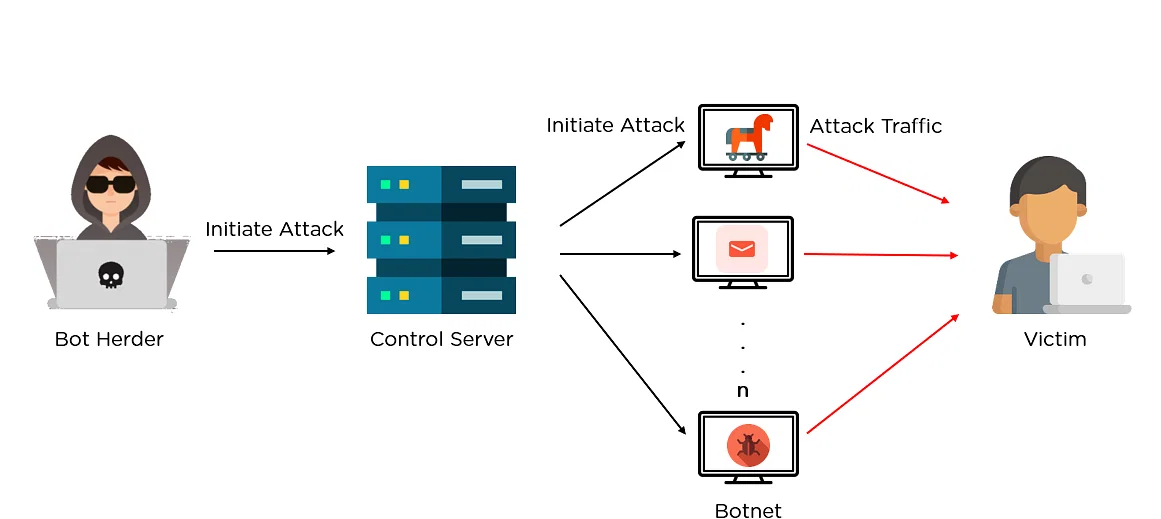
\includegraphics[width=8cm]{Botnet_1.jpg}
    \caption{esempio di architettura di una Botnet\cite{BotnetExampleImage}}
    \label{fig:botnetexample}
\end{figure}
Le Botnet possono essere di tipo \emph{push based} o \emph{pull based}. Nel primo caso è il server che invia i comandi al bot mentre nel secondo caso è il bot infetto che è incaricato di richiedere i comandi al server periodicamente.
 La modalità operazionale  dipende più che altro dal protocollo in uso\footnote{eg. HTTP costruito su modello richiesta-risposta quindi una botnet basata su questo protocollo sarà di tipo pull based}.
 Di seguito verranno presentati i principali schemi comunicazionali, topologie, protocolli e tecniche di occultamento delle Botnet \cite{vormayr2017botnet,vuong2011advanced}.


\section{Schema Comunicazionale}
Parte importante della comunicazione della botnet è il \emph{coordinamento}. I task che non sono automatizzati vengono eseguito solo dopo aver ricevuto l'apposito comando dal C\&C, il che implica una serie di messaggi da e verso il server. I task automatizzati non richiedono il coordinamento con il server di controllo e quindi non generano traffico di rete. Di conseguenza più sono i task automatizzati, meno sarà il traffico di rete necessario per la coordinazione del bot e più sarà difficile da identificare la botnet attraverso l'analisi del traffico di rete. Ovviamente limitare il coordinamento è a discapito della flessibilità, quindi solo una parte dei task viene automatizzata (ovviamente ci sono eccezioni anche a questo). 

Lo schema di comunicazione della botnet può essere separato in più parti: \emph{propagazione} e \emph{operazione}. Questi passi, dal punto di vista dell'host compromesso, possono avvenire solo sequenzialmente dato che l'infezione deve avvenire prima che il bot possa divenire operazionale. 
\subsection{Propagazione}
La parte di \emph{propagazione} é la fase in cui si cerca di reclutare nuovi bot. È la prima fase in nel ciclo di vita di un bot, ed è una fase importante dato che la potenza di una Botnet aumenta con la sua grandezza \footnote{eg. botnet capace di attacchi DDoS è più efficiente se ha più bot attraverso il quale generare traffico di rete}. Un'eccezione a questo sono gli APT (Advanced Persistent Threat) che sono attacchi mirati solitamente, e quindi necessitano solo di un limitato numero di macchine, oltre al fatto che devono rimanere nascoste nel sistema il più a lungo possibile, evitando dunque di propagarsi per non rischiare di essere rilevate.

La propagazione può avvenire attivamente o passivamente.
Entrambi i metodi di propagazione implicano che l'host vittima venga infettato con l'eseguibile di riferimento della  Botnet. 
\subsubsection{Attiva}
\label{PropagazioneAttiva}
Nella propagazione attiva, il bot cerca e sfrutta vulnerabilità in altre macchine per espandersi. Questo può avvenire su comando del C\&C o in automatico. A seconda dell'\textit{exploit}\footnote{codice usato per sfruttare una vulnerabilità} selezionato, una prima fase di scansione della rete può essere necessaria.


Una volta che la macchina è infetta, se il task non è automatizzato sarà necessario una messaggio di coordinazione dal C\&C server, in cui si specificano parametri per l'exploit e la possibile scansione di rete, oltre ad avviare l'infezione. Alcune Botnet mantengono questi parametri di configurazione in binario o in file separato, non necessitando dunque di un passo di coordinazione. 

La scansione di rete è opzionale, e può essere di diversi tipi a seconda delle informazioni che si vuole ottenere e del livello di occultamento che si vuole mantenere. Ad esempio potrebbero essere usate scansioni UDP\footnote{User Datagram Protocol}/TCP\footnote{Transmission Control Protocol} per cercare servizi esposti e vulnerabili, o semplicemente richieste ICMP\footnote{Internet Control Message Procotol} per limitarsi a identificare quali porte sono attive sull'host target.


Lo step principale é l'infezione, in cui si cerca di abusare i  servizi vulnerabili della macchina vittima. Questa fase dipende molto dal tipo di attacco scelto\footnote{eg. eseguire una richiesta contenente un payload maligno o eseguire attacco \textit{bruteforce}\footnotemark su un servizio (eg. \textit{ssh})}
\footnotetext{ attacco in cui si cerca di indovinare una combinazione in modo esaustivo, testando tutte le combinazioni possibili}.
Dato che durante questa fase la dimensione di dati scambiali é relativamente limitata, una fase ulteriore di \emph{download} può essere necessario.


\label{Download}Il download può avvenire in più parti, tipica delle \emph{multi stage infection}. In primo luogo la vittima esegue solo un piccolo eseguibile\footnote{un eseguibile di piccole dimensioni è solitamente meno sospetto} detto \emph{dropper} che si occupa di rimediare l'eseguibile vero e proprio dalla Botnet o da un'altra sorgente. Il binario può anche essere ricevuto criptato, rendendo ulteriormente difficile per i ricercatori riuscire a ottenere l'eseguibile per scopi di \emph{reverse engineering}\footnote{tecnica di analisi di un binario attraverso appositi strumenti, necessario per capire il flusso di esecuzione di un programma e relative funzionalità senza eseguirlo}. Quindi l'eseguibile viene opzionalmente decriptato ed eseguito.

La fase finale di questo processo di propagazione attiva è lo step di \emph{registrazione}.
Questo step è opzionale, ma fondamentale se si vuole tener traccia delle dimensioni della Botnet, in caso di Botnet \emph{push based}\footnote{il server deve conoscere la posizione del bot per poter comunicare con esso} o per particolari tipologie di Botnet\footnote{eg. botnet P2P}.

\subsubsection{Passiva}
Con propagazione passiva si intende la distribuzione del malware di riferimento attraverso altri vettori non in controllo della Botnet. Questo include propagazione attraverso email, siti web o dispositivi di archiviazione esterna. Comune a questi meccanismi di infezione è il fatto che la vittima infetta la propria macchina eseguendo il malware, attraverso un click o un azione particolare. 
La distribuzione via email può avvenire attraverso email di \emph{phishing}. Queste sono email che sembrano legittime, ma che in realtà hanno l'obiettivo di ingannare la vittima ad aprire un file allegato o visitare un particolare sito web maligno. Analoghi a email di phishing sono i siti web di phishing. Pagine web uguali alla loro copia legittima ma appartenenti a domini diversi (tecnica anche detta \emph{Domain typosquatting}).

Si possono anche usare vulnerabilità in browser o plugins della vittima o compromettere un sito web che esso visita frequentemente, per causare un \emph{drive by download}\footnote{tecnica di attacco che si riferisce al download non intenzionale di software maligno da sito compromesso}.

Si noti che in un contesto del genere, solo la ricezione di un email o la visita ad un sito web può essere individuata a livello di rete. Inoltre la comunicazione in questo caso usa gli stessi protocolli e modalità del traffico di rete legittimo. Per questo motivo solo attraverso Deep Packet Inspection \footnote{analisi dei pacchetti di rete che va oltre alla mera intestazione} (DPI) sarebbe possibile individuare contenuto eseguibile e questo è possibile solo se il tutto non è criptato.

Dispositivi di archiviazione esterna possono essere infettati per far sì che il malware si muova tra dispositivi. All'inserimento del media di archiviazione all'interno di un altro \textit{device}, questo avrebbe una copia dell'eseguibile potenzialmente eseguibile, senza alcun traffico di rete o movimenti sospetti.

Una volta che il malware viene eseguito sulla macchina vittima, seguono le fasi di download e registrazione, opzionali e comuni alla propagazione attiva (\Cref{PropagazioneAttiva}).


\subsection{Operazione}
 La seconda fase é quella \emph{operazionale} in cui si eseguono i veri e propri \emph{task}, a seconda di quali siano gli obiettivi della Botnet. I task possono essere categorizzati in accordo al loro obiettivo come: 
\begin{itemize}
    \centering
    \item Download  dati;
    \item Upload  dati;
    \item Forward Proxy;
    \item Reverse Proxy;
    \item Instruction.
\end{itemize}

\subsubsection{Download dati}
Con Download ci si riferisce alla memorizzazione di dati in bot, provenienti da sorgenti esterne. Dati possono essere file arbitrari, aggiornamenti della Botnet o malware aggiuntivo. I dati potrebbero perfino essere contenuti illegali atti a screditare la vittima. Questo meccanismo permette anche di offrire la Botnet come servizio di distribuzione di malware a pagamento. In questo modo sviluppatori di malware possono pagare il botmaster per avere un base di partenza di macchine su cui poter installare in modo agile il proprio software maligno.

La capacità di aggiornamento della botnet permette di adattare la rete a nuove necessità oltre che a difendersi da possibili minacce. Ovviamente questa capacità deve essere ben progettata in quanto può fornire un vettore di attacco a terzi, che possono sfruttare questa \textit{feature} per prendere possesso della Botnet o per rimpiazzarla con un altra.

L'operazione di Download inizia con una prima parte di coordinazione in cui si specifica quale file scaricare e dove cercarlo. Infatti il bot non è costretto a scaricare il file dal C\&C server, che quindi non necessita di incorporare meccanismi e protocolli di \textit{file transfer}. Il bot potrebbe avere all'interno del binario delle direttive di download da eseguire subito dopo l'infezione, rendendo la fase iniziale di coordinazione  superflua.
I dati possono anche essere passati all'interno del messaggio di coordinazione o essere inclusi in binario in fase di propagazione, in caso contrario verranno scaricati successivamente.

L'ultima fase è quella in cui si memorizzano i dati in macchina o dove si esegue il software aggiuntivo scaricato, a cui può seguire un messaggio opzionale verso il server.

\subsubsection{Upload dati}
L'operazione di Upload dati dal bot verso il server viene utilizzata da tutte quelle tipologie di Botnet che hanno come scopo ultimo la raccolta di dati o il calcolo distribuito.
Con raccolta di dati si intende prelevare informazioni dal sistema infetto. Queste informazioni possono essere file arbitrari, informazioni sensibili dell'utente, credenziali d'accesso, informazioni del sistema in uso, etc.
Con calcolo distribuito si intende l'upload del risultato di una computazione eseguita in modo distribuito su tutti i nodi infetti della rete.

Questo task inizia con uno step di coordinazione, in cui il C\&C server invia comandi con specifiche istruzioni o dati se necessari, che può essere opzionale nel caso l'upload venga eseguito subito dopo la propagazione. 
Successivamente i dati richiesti sono prelevati dal bot o la computazione richiesta è eseguita. 
Per concludere i dati sono inviati al server.
\subsubsection{Forward Proxy}
Un \emph{forward proxy} è un server capace di connettersi ad un  host specifico come tramite per un altro host.
Questo permette di mantenere l'anonimato dell'host che inizia la richiesta, di fare tunneling  delle connessioni o di effettuare connessioni verso host che altrimenti non sarebbero raggiungibili.

Le Botnet possono implementare proxy unidirezionali o bidirezionali. 
Proxy bidirezionali sono necessari se si vuole il risultato di una richiesta. Alcune Botnet includono SOCKS proxy \footnote{proxy server in grado di eseguire forward di connessioni TCP e UDP (da versione 5 in poi) indipendentemente dal protocollo applicativo veicolato}  come servizio, permettendo di utlizzare la Botnet come servizio di anonimato, sfruttando  i bot come proxy server generici.
Altro  uso di proxy bidirezionale è la possibilità di valicare Firewall o NAT infettandoli ed usandoli come proxy, fungendo da \textit{bridge} verso i device interni alla rete che altrimenti non sarebbero raggiungibili.

Per creare meno traffico sospetto possibile, la Botnet può anche usare i proxy per fare \emph{protocol encapsulation}, ovvero nascondere un protocollo all'interno di un altro. In questo modo i sistemi di rilevazione devono fare lo sforzo aggiuntivo di essere in grado di interpretare tutti i protocolli possibili se voglio ricostruire la comunicazione originale.

Proxy unidirezionali possono essere usati per effettuare attacchi DDoS. Infatti il botmaster non ha bisogno di controllare ogni messaggio e non è interessato alla risposta di questi. Gli basta comunicare destinazione e il tipo di comunicazione da utilizzare.

Un altro modo di usare i proxy unidirezionali è quello di usarli per distribuire email di spam. Durante la fase di coordinazione al  master basta invia il \textit{template} della email e una lista degli host da colpire.

A livello di schema comunicazionale, sia quello unidirezionale che bidirezionale iniziano con uno step di coordinazione.
Nel caso bidirezionale viene settata la configurazione del proxy con le porte su cui fare \textit{forwarding} e i protocolli da usare. Dato che queste configurazioni possono essere già incluse in binario questo step è opzionale.

Per il proxy unidirezionale invece, che è usato esclusivamente per eseguire task automatizzati, questo passo non è opzionale. Ad esempio se si vuole eseguire un attacco DDoS deve essere impostato il tipo di attacco, il target e la durata. Teoricamente queste informazioni possono essere incluse nel binario ma questo renderebbe inflessibile questo tipo di attacco che di per sé ha bisogno di essere improvviso e di durata variabile.

L'ultimo step é lo scambio di dati. In caso il proxy sia bidirezionale, la comunicazione sarà composta di richieste e risposte dove il bot farà da tramite.  Nel caso di proxy unidirezionale i dati sono inviati solamente da bot verso il target. 
\subsubsection{Reverse Proxy}
Le Botnet possono essere usate per creare un \emph{fast-flux network} (\Cref{fast-flux-network-label}). Un \emph{fast-flux network} consiste di più \emph{reverse proxy server}\footnote{mentre un forward proxy server funge da intermediario per un client, il reverse proxy server agisce come intermediario per il server, ponendosi tra il client e il server} che sono usati per connettersi al C\&C server.Dato che le connessioni sono verso i proxy, l'identità del C\&C server rimanere nascosta, rendendo il server più resistente a possibili \textit{take down}.

La comunicazione di rete necessaria per questo task inizia con uno step di coordinazione in cui il bot é istruito di quali porte aprire e verso quali indirizzi interni connettersi. Dopo questa fase di coordinazione altri host o bot possono connettersi al reverse proxy per comunicare indirettamente col C\&C server. Le informazioni di coordinazione non sono preinseribili nel binario del malware per via della natura della Botnet. I bot che fungono da reverse proxy potrebbero infatti  non essere mai raggiungibili  in uno scenario in cui gli indirizzi di questi dovessero essere prefissati\footnote{I bot potrebbero non essere online, il malware può essere neutralizzato o possono esserci problemi di rete.}.

\subsubsection{Instruction}
Una delle feature presenti nelle Botnet è la capacità di eseguire task a nome del botmaster che non generano traffico di rete. Esempi di task di questo genere sono: 
\begin{itemize}
    \item Terminazione di  altri processi;
    \item Canzellazione di  files;
    \item Modifiche al  traffico di rete dell'host;
    \item \textit{Disruption} di  servizi;
    \item Creazione di  \textit{backdoor}\footnote{rendere la macchina accedibile dall'attaccante attraverso la  rete };
    \item Distruzione o criptazione di dati in dispositivi di archiviazione;
    \item Esecuzione di eseguibili.
\end{itemize}

La comunicazione necessaria per questo genere di operazione inizia con una fase di coordinazione in cui vengono specificati il task da eseguire ed eventuali parametri. Gli eseguibili della Botnet possono essere accompagnati da files di configurazione contenenti queste istruzioni o possono essere inclusi in binario direttamente, rendendo questa fase opzionale. Ad esempio molte Botnet contengono una lista dei processi di anti virus da chiudere o disabilitare. Dopo lo step di coordinazione vengono eseguiti i comandi ricevuti.
\section{Topologie di rete}
La comunicazione tra C\&C server e i bot può essere organizzata da un punto di vista topologico nei seguenti modi:
\begin{itemize}
    \item Centralizzata;
    \item Decentralizzata;
    \item Ibrida.
\end{itemize}

\subsection{Centralizzata}
Nella topologia Centralizzata ogni bot si connette direttamente ad un unico server.
Per una topologia del genere spesso sono usati protocolli di comunicazione semplici come Internet Relay Chat (IRC) (\Cref{IRC}) o HyperText Markup Language (HTTP). Per questo motivo ne risulta anche semplificato il \textit{set-up}, dato che questi protocolli non hanno particolari esigenze da soddisfare. 
Una topologia del genere gode anche di bassa latenza, dato che bot e server si scambiano messaggi direttamente, e di alta scalabilità per via della semplicità della rete. 

Tuttavia questa semplicità di rete è a discapito della robustezza. Infatti una struttura centralizzata ha un singolo \textit{point of failuer} ed il \textit{take down} del server principale di comando e controllo comporterebbe la rottura dell'intera rete Botnet. 
Il singolo \textit{point of failure} può essere mitigato in parte utilizzando più C\&C server.
Un'altra tecnica utilizzata per mitigare il problema della robustezza è il \emph{fast-flux} che verrà descritto nella \Cref{fast-flux-network-label}.

Altro punto a sfavore di questa topologia è il fatto che gli indirizzi dei C\&C server devono essere inseriti all'interno del binario del bot. Questo é un rischio per il botmaster che potrebbe perdere il controllo del C\&C server in caso questi indirizzi dovessero essere scovati da un'analista di sicurezza informatica.
Una possibile soluzione potrebbe essere criptare od offuscare il codice del bot. Tuttavia anche questa soluzione risulterebbe temporanea in quanto non garantirebbe la sicurezza che questi indirizzi non vengano trovati a seguito di un analisi approfondita da parte di uno specialista.
Una tecnica spesso usata per evitare l'\textit{hardcoding} degli indirizzi dei server è il Domain Generation Algorithm (DGA) che verrà analizzato nella \Cref{DGA}.

\subsubsection{Fast-flux network}
\label{fast-flux-network-label}
In un Fast-flux network il servizio Domain Name System (DNS) di risoluzione degli \textit{hostname} viene usato come \textit{multiplexer} e \textit{load balancer}. La macchina infetta non comunica direttamente col server usando il suo indirizzo IP ma punterà a risolvere un hostname attraverso risoluzione DNS. Al record DNS in cui vi è registrato l'hostname da risolvere saranno associati molteplici indirizzi IP appartenenti a più bot della Botnet. Così facendo si sfrutta le capacità native di \textit{load balancing} dei server DNS per ciclare sugli indirizzi IP assegnati. I bot così associati a questo hostname sono gli unici a conoscenza dell'indirizzo IP del C\&C server e quindi sono gli unici in grado di comunicare con esso. 
Quando una macchina infetta ha necessità di comunicare con il server di controllo, risolve l'hostname associato ottenendo l'indirizzo IP di un bot che farà da proxy (reverse proxy) nella comunicazione verso il server.
In questo modo  si sposta il singolo point of failure dal server C\&C al DNS server.

Per rendere più complessa la rete ed eliminare anche questo point of failure si può creare un  \emph{double flux} network. Il \emph{double flux} usa lo stesso schema per ciclare i \textit{name server} autoritavivi che risolveranno l'hostname richiesto, traducendolo come visto in uno dei bot che farà da proxy verso il C\&C server. 

Si noti che registrare e de-registrare record DNS sono operazioni veloci e quindi è possibile variare velocemente i bot che fungono da proxy o name server.

Anche utilizzando questa tecnica rimane comunque il problema dell'hardcoding degli hostname all'interno del binario del bot. Per risolvere anche questo problema spesso  questa tecnica viene associata a \emph{Domain Generation Algorithm} (DGA) che verrà di seguito descritto.

\subsubsection{Domain Generation Algorithm (DGA)}
\label{DGA}
Domain Generation Algorithm é un algoritmo utilizzato per creare domini partendo da un valore di input variabile \cite{inproceedings}. Molte Botnet usano questo algoritmo per generare e registrare in automatico questi domini per il loro C\&C Server.

Quando il bot vuole cercare di contattare il server, usa l'algoritmo per generare un numero significativo di domini che proverà a risolvere. Il master che è a conoscenza dei dettagli dell'algoritmo, può preregistrare uno dei domini generati per essere contattato con successo dai bot.
Così facendo non è necessario pre~-~inserire domini all'interno dell'eseguibile.  Molti DGA usano il tempo corrente come input, rendendo necessario che ogni bot abbia l'orologio di sistema sincronizzato per poter funzionare correttamente. 
Se per esempio un bot dovesse generare 50.000 domini da testare, un ente governativo dovrebbe pre-registrare tutti i 50.000 domini per poter evitare che il botmaster riesca nel suo intento. Inoltre va considerato che se le comunicazioni tra bot e server dovessero usare cifratura a chiave pubblica, anche preregistrando correttamente uno dei domini che la Botnet usa per coordinare i bot, non si riuscirebbe a prenderne il controllo in quanto la comunicazione verrebbe negata per via delle firme digitali non combacianti con quelle del botmaster.

Un esempio di algoritmo DGA può essere il seguente:

\begin{algorithmic}[1]
    \State $i \gets 0$
    \State $domain \gets \:  '\;'$
    \State $year, month, day \gets getCurrentDate()$
    \While{$i<16$}
        \State $year \gets ((year \; ^  \wedge \; 8 \cdot year) >> 11) \; ^\wedge \; ((year \: \& \: \texttt{0xFFFFFFF0}) << 17) $
        \State $month \gets ((month   \;^ \wedge \; 4 \cdot month) >> 25) \; ^ \wedge \; 16 \cdot (month \: \& 
 \: \texttt{0xFFFFFFF8}) $
        \State $day \gets ((day \;^ \wedge \;(day << 13)) >> 19) \;^\wedge \; ((day \:\& \:\texttt{0xFFFFFFFE}) << 12) $
        \State $domain \gets domain + chr(((year ^\wedge month ^\wedge day) \% 25) + 97) $
    \EndWhile
\end{algorithmic}

\subsection{Decentralizzata (P2P)}
\label{TopologiaDecentralizzata}
Una topologia decentralizzata è tipica di una rete di soli bot dove ogni bot può essere un potenziale C\&C Server. Questo meccanismo in cui qualsiasi nodo può potenzialmente essere server è tipico delle reti Peer-To-Peer (P2P).
Ogni bot è connesso ad almeno un altro bot e i comandi del C\&C possono raggiungere ogni nodo della rete se ogni bot ha l'abilità di passare i comandi ai nodi direttamente connessi.


Una rete decentralizzata può essere a maglia parzialmente connessa o completamente connessa.

Una topologia a maglia completamente connessa ha il vantaggio di essere a bassa latenza dato che i comandi non devono essere passati a nodi intermedi per arrivare a tutti i nodi. Un altro vantaggio è che una rete del genere risulta molto robusta in quanto togliere un numero arbitrario di nodi non influenza negativamente la comunicazione di rete degli altri nodi. Tuttavia, considerando che questa topologia richiederebbe un altro numero di connessioni per una rete composta di molti nodi, risulterebbe non scalabile. I sistemi operativi infatti hanno limiti sul numero di connessioni che possono aprire e quindi viene limitato il numero massimo di bot in rete. Inoltre il numero di connessioni influisce sulla visibilità in rete della Botnet. Aggiungere e togliere nodi alla rete necessita di un alto numero di messaggi di coordinazione e per questo motivo spesso le Botnet P2P non sono a maglia completamente connessa.

Una topologia a maglia parzialmente connessa non ha i problemi delle topologie a maglia completamente connessa appena visti ma ha comunque dei fattori negativi. 
Dato che un bot non è connesso a tutti gli altri bot, l'eliminazione di nodi topologicamente importanti dalla rete può causare la completa interruzione delle comunicazioni per una parte dei device connessi.
Implementare topologie P2P risulta difficile a causa principalmente del dover garantire una distribuzione affidabile dei comandi verso tutti i bot oltre al problema di trovare i \textit{peers} iniziali.

Il problema della ricerca iniziale dei peers può essere ovviata inserendo la lista in eseguibile di bot. Un altro modo è quello di usare tecnologie pubbliche già esistenti per memorizzare ed in seguito reperire la lista di peers (eg. usare cache servers di applicazioni P2P esistenti). Il point of failure della rete si sposta così alla lista di peers iniziali. Un'altra alternativa alle liste di peers pubbliche è la possibilità di scansionare l'intera rete Internet in cerca di peers.

Dato che la rete non è a maglia completa, deve anche essere garantito il trasporto affidabile dei comandi che in questo caso non è nativo di questa topologia di rete. Per questo motivo spesso si usano protocolli P2P già noti che hanno questa funzionalità già implementata. Se si vuole creare la Botnet attraverso un protocollo \textit{ad-hoc}, le funzionalità di consegna affidabile dei messagi e di \textit{routing} devono essere implementate per poter garantire il corretto funzionamento della rete.

Dato che non tutte i dispositivi sono direttamente raggiungibili dall'Internet a causa di possibili Firewall o NAT, spesso le Botnet classificano i bot in due categorie: \emph{super node} e \emph{NAT-node}.
A seguito dell'infezione la connettività viene rilevata e solo i NAT-nodes sono usati per attività maligne mentre i super nodes sono usati solo come tramite per le comunicazioni con i bot C\&C.

\subsection{Ibrida}
Uno dei modi per ovviare alle problematiche di una rete decentralizzata e allo stesso tempo di fruire dei vantaggi che offre come topologia, è quello di combinarla con la topologia centralizzata per avere i vantaggi di entrambe.
Invece di connettere direttamente i bot al C\&C server, un livello di proxy viene aggiunto. Questo livello di proxy é costituito da bot connessi in P2P. 

I bot che eseguono i task costituiscono un ulteriore livello. 

L'assegnamento di un bot al ruolo di worker o proxy é eseguito considerando le proprietà di connettività dei bot analizzati.

Per aumentare ulteriormente la sicurezza del C\&C Server si potrebbe aggiungere un ulteriore livello di proxy a discapito di una maggiore latenza.

Altre  Botnet ibride sono possibili sfruttando topologie diverse per task diversi. Una Botnet potrebbe ad esempio sfruttare topologia P2P per lo scambio di messaggi e topologia centralizzata con un web server per il download di dati.

\section{Protocolli}
Di seguito verranno brevemente descritti i protocolli più comunemente usati a livello comunicazionale e operazionale nelle Botnet. 
\subsection{Protocolli Comunicazionali}
Con Protocolli comunicazionali si intende quei protocolli usati all'interno della Botnet per la comunicazione tra bot e Server, all'interno di una rete Centralizzata, o tra bot e bot all'interno di una Botnet P2P.
Ovviamente la scelta della topologia pone restrizioni sulle possibilità di scelta del protocollo comunicazionale.

Le Botnet spesso usano protocolli già esistenti, semplificando lo sviluppo della rete.

Il protocollo scelto può anche essere creato su misura. Questo permette di soddisfare  esigenze specifiche come un maggior mimetismo \footnote{eg. si potrebbe creare un protocollo che mimi il traffico legittimo}  o restrizioni di rete\footnote{eg. molte reti di corporazioni non permettono l'uso di particolari tipi di protocolli}.

\subsubsection{Internet Relay Chat (IRC)}
\label{IRC}
Internet Relay Chat  è un protocollo a livello applicativo di messaggistica \textit{text-based}, basato su architettura Client-Server. Venne inizialmente creato  per lo sviluppo di applicazioni chat su Internet \cite{rfc1459}, in particolare inizialmente usato su Bulletin Board System (BBS)\footnote{sistema telematico client-server creato negli anni '70 prima che i Web Browser venissero realizzati. L'utente si connetteva a un server centrale per condividere e prelevare risorse.}.
IRC inizia ad essere sviluppato nell'anno 1989. Nell'anno 1993 J.Oikarinen pubblica l'RFC 1459 in cui vengono pubblicate le specifiche del protocollo.

Il Client comunica con il Server che é responsabile di consegnare i messaggi ad altri client e server.
Messaggi possono essere scambiati  Client-Client o verso un gruppo di client attraverso \textit{canali}\footnote{gruppo di client a cui viene assegnato un nome. Un messaggio verso un canale arriva a tutti i client apparteneti al gruppo rappresentato.}. I canali possono essere protetti da password. 

Il protocollo supporta anche il trasferimento di file.

Questo protocollo facilita lo sviluppo di una Botnet basata su topologia Centralizzata. Il botmaster ad esempio potrebbe inviare i comandi verso un canale di bot, dove il C\&C in questo caso ricopre il ruolo di Server centrale incaricato di distribuire il messaggio a tutti i bot interessati. I canali come già detto, possono essere protetti da password per evitare che terzi prendano il controllo della Botnet. La capacità di file-transfer può essere sfruttata per distribuire malware, aggiornamenti della Botnet, file di configurazione, etc.

Tra gli svantaggi di questo protocollo ci sono il fatto che é facilmente identificabile e che non è un protocollo che viene comunemente usato nelle attività di tutti i giorni (nonostante sia un protocollo molto diffuso su Internet) e quindi potrebbe essere bloccato preventivamente via Firewall\footnote{Spesso questo è il caso delle reti corporative}.

\subsubsection{HTTP}
\label{HTTP}
Uno dei protocolli a livello applicativo più utilizzati su Internet. Usato per la trasmissione di pagine web da webserver a web client su Internet. È basato su architettura Client-Server dove la comunicazione di gruppo, al contrario di IRC, non è possibile. Vista il largo uso nella rete Internet, sono presenti tantissime implementazioni già pronte di client e server, rendendo lo sviluppo di una Botnet basata su protocollo HTTP facilitata.

Vista la struttura di HTTP può essere usato agilmente per creare una Botnet con topologia centralizzata.

Implementando un HTTP server e un HTTP client su ogni bot è possibile creare una rete P2P.
Nonostante questo sia possibile attraverso HTTP, si dovrebbe comunque risolvere alcuni dei problemi noti alle reti P2P come rendere la comunicazione tra bot affidabile e la gestione dei messaggi replicati.
Una possibile soluzione può essere creare dei \textit{layer di rete}   aggiuntivi sopra HTTP.
Si potrebbe creare quindi un livello P2P per aggiungere informazioni necessarie per il trasporto affidabile dei messaggi ad ogni nodo e per prevenire messaggi replicati.
Un altro livello di routing opzionale potrebbe essere implementato per gestire l'invio selettivo di un messaggio ad uno specifico bot non conoscendo il percorso esatto all'interno della rete P2P. Con il livello di routing si potrebbe anche implementare il trasporto affidabile, rendendo opzionale il livello P2P precedentemente descritto.


All'interno di questi livelli aggiuntivi si potrebbe anche aggiungere la possibilità di far rimbalzare il messaggio tra un numero arbitrario di nodi prima di consegnare il messaggio a destinazione, rendendo più complessa l'identificazione dell'origine del messaggio. Questa tecnica è nota col nome di Stepping Stones (\Cref{TecnicheOccultamento}).

Il fatto che HTTP sia largamente utilizzato su Internet rende lo scambio di messaggi attraverso questo protocollo non sospetto.

La sua variante  HTTPS permette l'uso di comunicazione HTTP all'interno di una connessione cifrata, rendendo quasi\footnote{i firewall posso usare una tecnica chiamata HTTPS-interception dove si sfrutta lo stesso principio degli attacchi Man In The Middle(MITM)\footnotemark{} \footnotetext{attacco informatico in cui l'attaccante si frappone tra la sorgente e la destinazione della comunicazione di rete, permettendogli potenzialmente di leggere/modificare/eliminare i pacchetti intercettati } per analizzare il contenuto dei pacchetti HTTPS} impossibile analizzare il contenuto dei messaggi da parte di strumenti di rilevazione.

\subsubsection{Server Message Block}
Server Message Block (SMB) é un protocollo  originariamente specificato da Microsoft, IBM e Intel per la condivisione di file, stampanti, porte seriali e comunicazioni di varia natura attraverso la rete \cite{SMB}.

Basato su architettura Client-Server. Un client si connette ad un server autenticandosi con crendenziali utente o come anonimo. Una volta connesso può richiedere una lista di \textit{shares} di sponibili. Con \textit{shares} si intende una lista di file o servizi accedibili.

SMB implementa anche meccanismi di comunicazione tra processi via network.

Questo protocollo può anche essere usato per infettare passivamente altri host. Se infatti un file condiviso è modificabile, un utente malintenzionato potrebbe inserire codice maligno all'interno di questo  che in seguito  potrebbe venir eseguito da un utente ignaro (propagazione passiva) in seguito al download  sulla propria macchina .

Questo protocollo spesso viene bloccato dai \textit{gateway} che provvedono accesso ad Internet, motivo per cui viene principalmente usato dalle Botnet come protocollo di comunicazione in rete locale.

\subsubsection{Protocolli P2P}
Come già detto nella sezione inerente le topologie decentralizzate di Botnet (\ref{TopologiaDecentralizzata}), i protocolli P2P esistenti vengono spesso adottati per evitare di dover sviluppare protocolli P2P da zero. Questi protocolli possono  essere usati per creare una rete P2P separata o per nascondere la rete di bot all'interno di una rete P2P esistente.
Un esempio di protocollo usato è WASTE \cite{WASTE}, originariamente creato come protocollo di messaggistica distribuita e file sharing. Un altro esempio di protocollo usato è Kademlia \cite{maymounkov2002kademlia}, che gestisce la struttura della rete, la comunicazione tra nodi e il modo in cui lo scambio di informazioni è effettuato.

\subsubsection{Protocolli ad-hoc}
La creazione di un protocollo \textit{ex novo} permette di creare una comunicazione su misura che rispecchi le esigenze e gli obiettivi che la Botnet vuole perseguire. 

La maggior parte dei protocolli creati appositamente risulta basata su UDP o TCP a livello di trasporto. Ci sono anche casi osservati di protocolli basati su ICMP. Come già discusso precedentemente a seconda della topologia scelta  si devono implementare tutte le accortezze necessarie al corretto funzionamento della rete. 

Se si desidera una rete P2P è necessario implementare la comunicazione affidabile dei messaggi e gestire i messaggi duplicati. La questione dei messaggi duplicati può essere ovviata associando un ID ai comandi.
Il trasporto affidabile dei messaggi deve essere gestita anche nel caso si utilizzi UDP come protocollo a livello di trasporto. Questo può essere garantito ad esempio implementando ritrasmissione dei messaggi e l'invio di acknowledgments.
Un protocollo basato su UDP con consegna affidabile dei messaggi avrebbe anche il vantaggio di poter permettere più connessioni contemporaneamente in quanto nessuna connessione deve essere mantenuta al contrario di TCP.

Il payload dei messaggi può essere in binario o testo. Un payload formato testo necessita di un \textit{parser} per comprendere i comandi così codificati, oltre a essere più facile da analizzare a livello di reverse engineering.

Uno dei punti a sfavore dei protocolli creati su misura é che questi non sono usati all'interno di traffico di rete legittimo e quindi potrebbe essere identificato.

\subsection{Protocolli Operazionali}
Oltre ai protocolli usati per il normale funzionamento della Botnet, sono necessari anche altri protocolli per svolgere i task operazionali atti a  raggiungere l'obiettivo preposto. 
Di seguito verranno presentati alcuni esempi di  protocolli usati per le più comuni attività  di una Botnet:

\begin{itemize}
    \item Per inviare spam via email deve essere in grado di poter usare  Simple Mail Transport Protocol (SMTP). SMTP é un protocollo Client-Server usato per inviare messaggi di posta elettronica attraverso server dedicato (Server SMTP). Dato che molti server di posta elettronica richiedono autenticazione solo per inviare messaggi fuori dalla rete locale, questa risulta la principale causa di spam. Un bot potrebbe infatti sfruttare la sua posizione all'interno della rete per inviare emails di spam attraverso il mail server comune, verso altri nodi della rete locale. Per questo motivo molti email providers bloccano email provenienti da IP di reti private;
    \item HTTP e HTTPS vengono usati per eseguire \textit{click fraude}, ovvero simulare il click su un URL o  annuncio pubblicitario col fine di alterarne le statistiche di visita della risorsa. In questo modo il botmaster può fare profitto grazie al numero falsato di visite all'annuncio o pagina web;
    \item HTTP, UDP e TCP vengono anche usati per eseguire attacchi DDoS in cui si cerca di sovraccaricare il network del servizio target. Un altro modo di sovraccaricare il servizio è attraverso l'invio di richieste computazionali intensive con l'intento di saturare la capacità di calcolo dell'applicazione target.
\end{itemize}


\section{Tecniche di occultamento e offuscamento di comunicazione}
\label{TecnicheOccultamento}
Di seguito verranno brevemente raccolte alcune delle tecniche usate dalle Botnet per nascondere le comunicazioni od offuscarne il contenuto. Con offuscamento si intende rielaborare il contenuto in modo che risulti complesso comprenderne il significato, usato spesso per rendere più difficili i tentativi di reverse engeneering o di analisi.

\subsection*{Canali nascosti}
 Considerando che, come  già detto, i protocolli costruiti ad-hoc sono facilmente individuabili in quanto non figurano comunemente nella rete Internet e che i protocolli già esistenti generano traffico di rete che non dovrebbe esistere in scenario normale,  si possono usare i canali nascosti per occultare la comunicazione.
  Con canali nascosti si intende instaurare una comunicazione sfruttando mezzi che non sono usati a scopo comunicativo. Un esempio è usare gli header dei segmenti TCP o dei datagrammi del protocollo IP per comunicare informazioni o comandi. 

 \subsection*{Crittografia}
 L'ispezione del contenuto del traffico di rete permette la ricerca di pattern di messaggi  di Botnet conosciute, portando ad una possibile identificazione dei device infetti o del C\&C server. 
 Per questo motivo spesso le Botnet usano crittografia a livello di rete per fare in modo che terzi non riescano a ispezionare il contenuto delle comunicazioni. 

 Un esempio di protocolli usati a tal fine sono HTTPS o TLS. Sebbene sia possibile creare protocolli crittografici su misura, ciò pone il rischio che una falla nel protocollo crittografico lo renda completamente inefficace. Per questo motivo i botmaster devono preoccuparsi di usare protocolli aggiornati che non presentino vulnerabilità note nel caso decidano di utilizzare protocolli già esistenti.

 \subsection*{Molteplici protocolli}
 Per adattare il bot alla rete in cui risiede e quindi rendere la Botnet meno identificabile è possibile creare un livello di rete variabile capace di usare molteplici protocolli. Avendo una vasta scelta di protocolli, il bot potrebbe scegliere di usare quello più popolare all'interno della rete in cui risiede per rendere la comunicazione meno sospetta.

 \subsection*{Compressione}
 La compressione dei dati viene comunemente usata per ridurre la dimensione di files. Tuttavia nel comprimere i dati ne offusca anche il contenuto in quanto, nonostante l'informazione originaria rimanga intatta all'interno dei dati compressi, questi risultano non interpretabili a meno di conoscer l'algoritmo di decompressione.
 
 Dato che questa tecnica non richiede alcuna chiave, chiunque conosca l'algoritmo di compressione può  decomprimere i dati e quindi risalire al contenuto originario.

 \subsection*{Steganografia}
 La steganografia é un'altra tecnica di offuscamento. Essa consiste nel nascondere informazioni all'interno di \textit{contenitori} che non sono pensati per la comunicazione. Simile a livello di logica ai \emph{canali nascosti} ma che usa files (eg. immagini,video,documenti,etc.) per comunicare al posto degli attributi dei  pacchetti di rete.

 In passato sono state proposte Botnet capaci di sfruttare questo principio all'interno dei social network, incapsulando le informazioni dei comandi all'interno di immagini JPEG postate dall'utente \cite{nagaraja2011stegobot}.

 Altri esempio peculiare di Botnet di questo tipo é quella ideata da A.Compagno e collaboratori, che hanno sfruttato i messaggi di testo all'interno dei social network, usando caratteri non visualizzati dai web browser \cite{nagaraja2011stegobot}.


 \subsection*{Stepping Stones}
 
 Tecnica usata per aumentare la segretezza del C\&C server che consiste nell'aggiungere un numero arbitrario di nodi intermedi tra il server e i bot destinatari dei comandi.  Questo può essere ottenuto implementando un layer di routing che permette di far rimbalzare i messaggi tra un numero desiderato di nodi prima di consegnarlo a destinazione.














 

\chapter{Infrastruttura di testing}
Prima di poter analizzare le Botnet dinamicamente, è necessario progettare ed eseguire il \textit{deploy} di un infrastruttura  sicura, in cui è possibile eseguire i malware relativi alla Botnet oggetto di studio senza rischiare di compromettere dispositivi al di fuori del perimetro designato.


Il deploy dell'infrastruttura è stato eseguito su un Server VMWare eSxi (\ref{esxi})  raggiungibile attraverso Virtual Private Network (VPN), in quanto situato all'interno della rete del campus Universitario di Cesena. Attraverso le capacità di virtualizzazione del server sono state create una macchina Linux per ospitare il C\&C server e due macchine che verranno infettate con malware per trasformarli in bot attivi. Le macchine bot in questione sono una basata su Linux e l'altra su Windows.  Queste macchine sono assegnate ad una rete VLAN isolata così che non siano in grado di comunicare con altri dispositivi al di fuori delle macchine soggette al test. Chiameremo questa rete \emph{Botnet Vlan}.

Per far in modo che le macchine sotto testing potessero occasionalmente interfacciarsi alla rete Internet in modo controllato è stato aggiunto un Firewall (\ref{firewall}). La macchina in questione usa  ClearOs (\ref{ClearOS}) come sistema operativo e ha due Network Interface Card (NIC).
Una delle NIC è collegata ad una VLAN connessa a Internet e ha indirizzo IP assegnatogli attraverso Dynamic Host Configuration Protocol (DHCP). L'altra NIC è collegata alla Botnet Vlan e ha indirizzo IP statico assegnatogli manualmente. 

Una volta configurato il Firewall, le tabelle di routing dei bot e del C\&C server sono state modificate per fare in modo che il Firewall operasse da gateway per questi dispositivi. In questo modo quando i dispositivi all'interno della Botnet Vlan cercheranno di comunicare all'esterno della rete il Firewall filtrerà le comunicazioni.

ClearOS ha diversi moduli installabili per configurare le funzionalità di Firewall. In questo caso è stato utilizzato un modulo basato su Iptables (\ref{iptables}).
    
Oltre alle funzioni di Firewall sono state usate le funzionalità di server DHCP che il sistema operativo offre attraverso modulo dedicato. Per mezzo di  questo sono stati assegnati gli indirizzi IP alle macchine interne alla Botnet Vlan.

In seguito alla conferma della connettività  Internet delle macchine interne alla Botnet Vlan,  sulle macchine Linux è stato installato per comodità un ambiente Desktop , di cui erano privi.

In fine per velocizzare il deploy dei nodi della Botnet nelle rispettive macchine  e per facilitare il testing è stato installato Docker all'interno delle macchine della VLAN Botnet.

Per lo scambio di file con macchine fuori dal perimetro del server eSXI è possibile usare SSH Tunneling, a patto che il dispositivo interessato sia connessa alla stessa VPN del server.
    
Di seguito verranno descritte più nel dettaglio le principali tecnologie sopra citate.

\section{Server VMWare ESXi}
\label{esxi}
Il server sul quale sono stati effettuati i test usa  ESXi (Elastic Sky X integrated) \cite{esxi} sviluppato da VMWare come \emph{hypervisor bare metal} per la creazione e  gestione di macchine virtuali.


Un hypervisor, anche conosciuto come \textit{virtual machine monitor}, è un tipo di software di virtualizzazione che supporta la creazione e il management di macchine virtuali \cite{desai2013hypervisor,techtargetHypervisor}. Consente ad un computer host di supportare diverse \textit{guest Virtual Machine (VM)}  , condividendo le risorse come memoria e potenza di calcolo.
Ha il compito di astrarre il lato software di un computer dal suo hardware traducendo richieste da risorse fisiche a virtuali.
L'hypervisor tratta le risorse di elaborazione ( tra cui CPU, memoria, \textit{storage}) come un pool di risorse facilmente riposizionabili tra i guest esistenti o su nuove VM.
A seconda delle esigenze le risorse vengono suddivise e trasferite dall'ambiente fisico alle varie macchine virtuali. Durante l'esecuzione di una VM, quando un utente o un programma invia un'istruzione che richiede ulteriori risorse dall'ambiente fisico, l'hypervisor programma la richiesta in base alle risorse del sistema fisico, in modo che il sistema operativo e le applicazione della macchina virtuale possano accedere al pool condiviso di risorse fisiche.

Esistono due tipi di hypervisor:
\begin{description}
    \item[tipo 1 o \textit{bare metal}] come un leggero sistema operativo che esegue direttamente sull'hardware di macchina host
    \item[tipo 2 o \textit{hosted}] livello software  che viene eseguito  sopra un sistema operativo già funzionante, come una normale applicativo.
\end{description}

Le principali differenze tra questi sono che l'hypervisor di tipo 1 è installato nell'unità di archiviazione della macchina host ed esegue direttamente sull'hardware come farebbe un sistema operativo, mentre il tipo 2 è installato come un normale software ed esegue sopra un sistema operativo di cui sfrutta le capacità di virtualizzazione.
L'hypervisor bare metal risulta essere più sicuro in quanto non in contatto con il sistema operativo. Infatti in caso di malfunzionamento del sistema operativo o in caso risulti vulnerabile a possibili attacchi comprometterebbe la sicurezza dell'intera struttura virtualizzata.

Inoltre i \textit{tipo 1} risultano più efficienti e veloci in quanto le richieste di risorse tra hardware e hypervisor non devono passare attraverso il livello aggiuntivo del sistema operativo che ne fa da tramite.

ESXi offre anche  capacità di virtualizzazione di rete \cite{esxiVirtualNetwork}.
Attraverso la virtualizzazione di rete, è possibile creare reti virtuali di macchine che utilizzino gli stessi protocolli delle reti fisiche, sia all'interno di un singolo host ESXi Server che tra diversi host, per scopi di sviluppo, testing o per deployment in produzione. 
Le componenti principali della rete virtualizzata di ESXi sono i virtual switch e i virtual adapter.
I virtual switch permettono alle macchine virtuali all'interno di un singolo host di comunicare tra loro senza la necessità di hardware di rete aggiuntivo, utilizzando gli stessi protocolli degli switch fisici. Inoltre, gli switch virtuali di ESXi  supportano le VLAN, compatibili con le implementazioni standard dei vendor di terze parti.  Ogni macchina virtuale può essere configurata con uno o più adattatori Ethernet virtuali, ognuno dei quali ha un proprio indirizzo IP e MAC, conferendo alle macchine virtuali le stesse proprietà di quelle fisiche dal punto di vista della rete.


\section{Firewall}
\label{firewall}
Un Firewall è un dispositivo per la sicurezza di rete che permette di filtrare il traffico in entrata e in uscita in base a regole prestabilite dall'utente \cite{krit2017overview}.
Costituiscono una barriera tra le reti interne, sicure e controllate, e le reti esterne che possono essere affidabili o meno. 
In questo caso il Firewall verrà usato per l'esatto opposto, col fine ultimo di salvaguardare la rete esterna. Infatti è la rete interna che sarà considerata pericolosa in quanto sarà popolata da host infetti potenzialmente in grado di espandere l'infezione in rete.

Un Firewall può essere costituito da un componente hardware, software o entrambi.
Tra i diversi tipi di Firewall ci sono:
\begin{description}
    \item[Packet filtering] È il tipo di Firewall più comune, anche chiamato \textit{network layer firewall} o \textit{stateless firewall}. Tratta ogni frame o pacchetto individualmente, accettandolo o negandolo all'interno del network di destinazione in base a regole prestabilite. Tra i criteri che è possibile comparare con le informazioni dei pacchetti ci sono: tipo di protocollo, indirizzo sorgente o destinazione, porte di origine o destinazione, direzione del traffico, etc.;
    \item[Circuit-level gateway] Monitora  l'\textit{handshake} TCP tra l'host locale e quello remoto per determinare se la sessione che sta per essere inizializzata è legittima in base all'affidabilità del sistema remoto. Non ispeziona i pacchetti di sua iniziativa. Applica meccanismi di sicurezza quando si stabilisce una connessione. Una volta che questa è stabilita i pacchetti possono fluire senza ulteriori controlli. Il server che riceve richieste filtrate da questo Firewall vedrà nei messaggi di rete le informazioni del Firewall e non quelle del client originario, nascondendone l'identità;
    \item[Statefull filters] Mantiene traccia di tutte le connessioni che passanno attraverso esso e può determinare se un pacchetto è l'inizio di una connessione, parte di una connessione già stabilita, o un pacchetto invalido. A tal scopo tiene un record in \textit{cache} per ogni connessione aperta. Quando il primo pacchetto di una nuova connessione occorre, il Firewall ne compara le informazioni con delle regole prestabilite e su questa base decide se bloccare o accettare la connessione con i relativi pacchetti;
    \item[Application layer] Un Application Layer Firewall, anche chiamato Application proxy Firewall, protegge le risorse di rete filtrando messaggi a livello applicativo. Più complicato di un \textit{pachet filtering Firewall} in quanto esso è in grado di comprendere il protocollo applicativo e i dati, oltre a poter intercettare ogni informazione destinata all'applicazione. Sulla base delle informazioni disponibili per prendere decisioni, può autenticare utenti e giudicare se dati che dovrebbero fluire possono presentare una possibile minaccia. Combina alcune degli attributi del packet filtering Firewall con quelli del circuit level  gateway Firewall. Capace di filtrare pacchetti non solo per i protocolli  a cui è destinato ma anche sulla base di altre caratteristiche.

    L'application proxy Firewall viene detto proxy service mentre la macchina host che li esegue viene chiamato \textit{application gateway}.

    Anche se risulta più sicuro di altre soluzione Proxy, può impattare negativamente la performance di rete;
    \item[Multilayer inspection] Questo tipo di firewall è in grado di analizzare i pacchetti a livello di rete, trasporto e applicazione, offrendo un elevato livello di controllo sul traffico di rete. Inoltre, il firewall multilayer inspection è in grado di mantenere lo stato dei pacchetti , ovvero di ricordare a quali connessioni appartengono, in modo da consentire un controllo più preciso su quali pacchetti vengono autorizzati a passare attraverso il firewall, in modo analogo agli statefull Filters Firewall.


\end{description}
Navigando sul web si possono trovare numerose tecnologie atte allo scopo. In questo caso è stato scelto ClearOS come sistema operativo capace di eseguire le funzionalità di filtraggio del traffico di rete. 
\subsection{ClearOS}
\label{ClearOS}
ClearOS \cite{clearos} è un sistema operativo open source basato su CentOS. Ideato per le piccole medie imprese che vogliono soluzioni flessibili. ClearOS offre diverse capacità tra cui Intrusion Detection, Content Filter, Firewall, Bandwith Management, Domain Controller, Mail Server, DNS Server, NAT, DHCP Server, Web Server, e molto altro.
Il punto forte di ClearOS è la facilità di utilizzo oltre alla flessibilità. Tutte le capacità di questa piattaforma sono distribuite sotto forma di moduli scaricabili al bisogno attraverso una comodissima web GUI. Oltre ai moduli gratuiti, ClearOS offre soluzioni a pagamento più adatte al mondo \textit{enterprise}. In questo modo l'azienda interessata può comprare solo i moduli che desidera ed espandersi al bisogno acquistando ulteriori moduli. 

Una volta installato, configurato e impostato come gateway all'interno della Botnet Vlan, é stato installato il modulo aggiuntivo di Server DHCP, per configurare in automatico gli indirizzi di rete delle macchine interne alla Vlan.
In seguito è stato anche testato il modulo DNS, che in fase di testing non è stato utilizzato in quanto i dispositivi in rete venivano referenziati per indirizzo IP, e alcuni moduli gratuiti di Intrusion Detection System (IDS). Tuttavia i moduli di IDS gratuiti non sono stati ritenuti all'altezza del compito che avrebbero dovuto svolgere e sono stati quindi disinstallati. Va comunque considerato che non sono state testate le soluzione a pagamento che sicuramente sarebbero state più adatte al contesto. 
In fine prima di selezionare un modulo Firewall tra le opzioni disponibili offerte da  ClearOS, sono stati studiati Netfilter (\ref{netfilter}), Iptables (\ref{iptables}), Nftables (\ref{nftables}) e Firewalld (\ref{firewalld}). Una volta comprese queste tecnologie é stata scelta una soluzione (modulo) basata su Iptables.

Attraverso il modulo di Firewall sono state scritte delle regole, con sintassi uguale a quella di Iptables, per le seguenti security policies:\begin{itemize}
    \item Non permettere traffico ipv6 da,verso,attraverso il Firewall;
    \item Permetti traffico  da e verso la web GUI del Firewall;
    \item Permetti traffico  DHCP da e verso il Firewall;
    \item Permetti traffico  DNS da e verso il Firewall;
    \item Permetti traffico  SSH da e verso il Firewall;
    \item Permetti traffico da e verso gli Intrusion Detection Systems\footnote{la macchina con ClearOS è stata utilizzata per comodità come  punto di interfacciamento con la web GUI del Firewall e le web GUI degli IDS così che si potesse avere il controllo della rete attraverso un unico web browser};
    \item Nega tutto il traffico non precedentemente permesso da/verso/attraverso il Firewall.
\end{itemize}

Quando era necessario connettere le macchine della Vlan ad Internet, venivano disattivate le regole opportune per permettere il traffico di rete. 

\subsection{Netfilter}
\label{netfilter}
Netfilter \cite{netfilter,netfilterAndIptables} é un framework per kernel Linux 2.4.x e superiori, che permette di intercettare e manipolare i pacchetti di rete. Attraverso Netfilter è possibile realizzare diverse funzionalità di rete tra cui:
\begin{itemize}
    \item Stateless firewall;
    \item Statefull firewall;
    \item Tutti i tipi di traduzione di indirizzi IP o porte (eg. NAT) .
\end{itemize}
Attraverso gli \textit{hook} di Netfilter i moduli del kernel possono registrare funzioni di \textit{callback} in diverse posizioni chiave lungo il Linux network stack. Quando un pacchetto progredisce attraverso lo stack  (in entrata o in uscita), al raggiungimento di uno di questi punti chiave, l'hook associato a questa posizione specifica si attiverà, chimando le funzioni di  callback dei moduli kernel registrati presso di esso.
In particolare gli hooks sono:
\begin{description}
    \item[NF\_IP\_PRE\_ROUTING] Questo hook verrà attivato da qualsiasi pacchetto in entrata subito dopo essere entrato nello stack di rete. Questo hook viene elaborato prima che venga presa qualsiasi decisione di instradamento relativa a dove inviare il pacchetto;
    \item[NF\_IP\_LOCAL\_IN] Questo hook verrà attivato dopo il routing di un pacchetto in ingresso, se il pacchetto è destinato al sistema locale;
    \item[NF\_IP\_FORWARD] Questo hook verrà attivato dopo il routing di un pacchetto in ingresso, se il sistema deve eseguire il forward del pacchetto;
    \item[NF\_IP\_LOCAL\_OUT]  Questo hook verrà attivato da qualsiasi traffico in uscita dal sistema locale, nel momento in cui netra nel network stack;
    \item[NF\_IP\_POST\_ROUTING] Questo hook verrà attivato da qualsiasi traffico in uscita o se il sistema deve fare il forward del pacchetto, dopo che il routing è avvenuto e prima che il pacchetto venga spedito in linea.
\end{description}
\begin{figure}[hbtp]
    \centering
    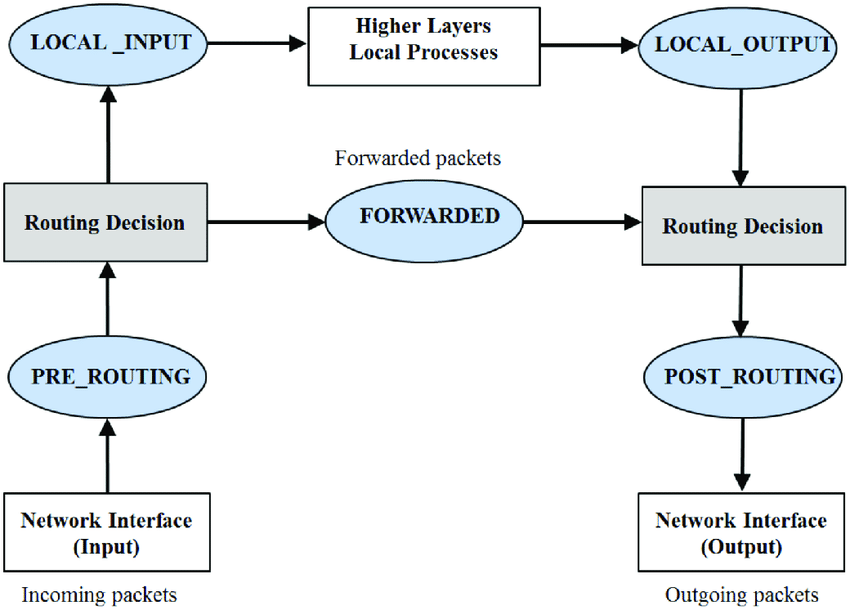
\includegraphics[width=8cm]{netfilter_hooks.png}
    \caption{Flusso del pacchetto attraverso il Linux network stack con Netfilter hooks \cite{NetfilterHooks}}
    \label{fig:netfilter_hooks}
\end{figure}
I moduli kernel registrati in questo modo, possono assegnare un numero di priorità per identificare deterministicamente in quale ordine verranno eseguite le funzioni di callback.

Quando una funzione di callback viene eseguita, il modulo può decidere di alterare il pacchetto responsabile dell'esecuzione della funzione. Al termine dell'esecuzione, inoltra al framework la propria decisione sul futuro del pacchetto. Il pacchetto può quindi essere scartato, ignorato, inserito in coda per poter essere maneggiato da software che appartengono allo \textit{spazio utente}\footnote{Netfilter è un framework che esegue a livello di kernel  in kernel mode e quindi l'utente che esegue software in user mode non potrebbe interagire direttamente con questo}, o potrebbe proseguire il suo corso attraverso lo stack.

Per interagire con il framework Netfilter dunque è necessario sviluppare un modulo kernel che possa registrare funzioni di callback presso gli hooks o scrivere un applicativo che interagisca con la coda nello spazio utente (user mode).

Per semplificare il processo e non dover specificatamente scrivere un software per  filtrare  i pacchetti spesso si usano programmi come Iptables e Nftables. Attraverso questi software é possibile definire insiemi di regole di filtraggio dei pacchetti.

\subsection{Iptables}
\label{iptables}
Iptables usa tabelle per organizzare queste regole. Nello specifico le tabelle \textit{built-in} di Iptables sono:
\begin{description}
    \item[Filter Table] Per controllare il flusso dei pacchetti che entra ed esce dal sistema;
    \item[NAT Table] Per ridirigere connessioni verso altre interfacce di rete;
    \item[Mangle Table] Per modificare headers di pacchetti;
    \item[Raw Table] Provvede meccanismo per marcare pacchetti ed escluderli dal tracking di connessione\footnote{ Netfilter  riesce ad identificare un pacchetto come parte di una connessione e Iptables quindi sfrutta questa capacità in automatico};
    \item[Security Table] Usata per interagire con SELinux\footnote{Security Enhanced Linux é un modulo di sicurezza del Kernel Linux che fornisce insieme di strumenti di sicurezza}.
\end{description}
Ogni tabella è a sua volta organizzata in \textit{chains} che contengono le vere e proprie regole. Mentre le tabelle rappresentano lo scopo generale delle regole che contengono, le chains rappresentano i Netfilter hooks a cui si riferiscono e da cui vengono attivati. Le chains quindi determinano quando le regole al loro interno verranno valutate.
I nomi delle chains fanno riferimento ai nomi degli hooks a cui sono associati e sono:
\begin{itemize}
    \item Prerouting;
    \item Input;
    \item Forward;
    \item Output;
    \item Postrouting.
\end{itemize}

Dato che alcune operazioni/decisioni hanno senso solo in alcuni punti del network stack, non ogni tabella ha tutte le precedenti chains registrate presso i rispettivi Netfilter hooks. Ad esempio la Filter Table hanno solo le Input,Output e Forward chains registrate.

Come detto le regole sono posizionate all'interno delle chain delle tabelle specifiche. Quando una chain è chiamata dal rispettivo hook, i dettagli del pacchetto vengono comparati con le regole con ordine. Ogni regola è divisa in due parti.
La prima parte è quella interessata dei criteri di match con le informazioni del pacchetto. Tra i criteri di match ci sono il protocollo usato, la sorgente, la destinazione, lo  stato della connessione, le porte utilizzate, e molto altro.
La seconda parte invece detta \textit{target} specifica un azione da compiere sul pacchetto. Tra i target più comuni ci sono Accept, Reject, Drop e Jump.

Oltre alle chains built-in è anche possibile creare chains personalizzate. Queste non sono associate ad   hook Netfilter e sono raggiungibili solo attravers il target Jump, ovvero saltando da una chain built-in a questa. Quando un pacchetto esegue il match con una regola avente target Jump, il controllo può saltare all'interno di chains definite dall'utente. In caso  non vi sia match all'interno di queste, il controllo tornerebbe alla chain d'origine. In questo modo è possibile aumentare l'organizzazione del sistema. 

\subsection{Nftables}
\label{nftables}
Nftables \cite{nftables} è il successore di Iptables, basato anch'esso sul framework Netfilter. Risulta più flessibile, scalabile ed efficiente nel classificare i pacchetti.
La struttura é uguale a quella di Iptables, ovvero è composto di tables, che contengono chains, che a loro volta contengono regole.
Tra i vantaggi che offre rispetto a Iptables ci sono:
\begin{itemize}
    \item Una singola regola può avere più targets mentre Iptables può averne solo uno per regola;
    \item Possibilità di creare regole più complesse attraverso strutture dati come maps, sets, concatenazioni, diminuendo quindi il numero di regole da controllare e quindi aumentando l'efficienza;
    \item Non ha tables e chains predefinite, sfrutta combinazione di parametri selezionabili come il tipo di hook e lo scopo per determinarne il comportamento;
    \item Più facile da configurare;
    \item Possibilità di gestire regole IPv4 e IPv6   attraverso lo stesso tool, mentre in Iptables le configurazioni sono gestite separatamente\footnote{viene usato  tool iptables per le configurazioni IPv4 e ip6tables per quelle IPv6}.
\end{itemize}

\subsection{Firewalld}
\label{firewalld}
Firewalld \cite{firewalld} è uno stumento di gestione del Firewall che sfrutta  Nftables o Iptables. È il tool di gestione Firewall predefefinito di RHEL 7, CentOS, Fedora ed altre distribuzioni Linux. Esso agisce come  un'interfaccia front-end e non è quindi un Firewall \textit{stand-alone}.
Firewalld è strutturato in zone. Le interfacce di rete o range di indirizzi IP possono  essere assegnati a zone specifiche. Una zona  dichiara quali porte o servizi sono permessi o bloccati, oltre a poter definire ulteriori regole più complesse. Le zone sono formulate come file XML e sono posizionate all'interno della directory di Firewalld.
Il funzionamento alla base di Firewalld è indipendente dal fatto che venga utilizzato Nftables o Iptables. Al boot esegue uno script Python che converte e carica le regole, configurate con Firewalld, in Nftables o Iptables . Sono anche disponibili interfacce grafiche che ne semplificano ulteriormente l'utilizzo.

\section{Docker}
\label{docker}
In uno scenario di normale sviluppo di un'applicazione \textit{end-to-end}, dove si vogliono utilizzare diversi servizi che devono cooperare tra loro, ci possono essere le seguenti problematiche da tenere in considerazione:
\begin{description}
    \item[Compatibilità/dipendenze] I diversi servizi dell'applicativo possono richiedere differenti versioni della stessa libreria. Le librerie devono essere compatibili con il sistema operativo e l'hardware sottostante. Inoltre queste hanno dipendenze che devono essere soddisfatte;
    Il problema di soddisfare tutte queste esigenze contemporaneamente per permettere il corretto funzionamento dell'applicativo è conosciuto come \textit{Matrix~from~Hell};
    \item[Tempi di Setup] La configurazione di un nuovo ambiente di sviluppo da zero sottointende che lo sviluppatore debba assicurarsi di avere il giusto sistema operativo e le librerie necessarie nelle versioni corrette, e che le dipendenze siano risolte correttamente. Questo processo può essere laborioso e non banale,  oltre che richiedere una considerevole quantità di tempo;
    \item[Differenti ambienti di sviluppo] Essendoci diversi ambienti di sviluppo, test e produzione, non è detto che, una volta completata una modifica,  l'applicativo funzioni correttamente quando viene eseguito in un ambiente differente.
\end{description}

Questi sono alcuni dei motivi per cui può essere utile containerizzare i servizi.
Con containerizzazione si intende raggruppare  il codice software e tutti i relativi componenti necessari, come librerie, framework e altre dipendenze, in modo che risultino isolate in un proprio contenitore, detto \emph{Container} .

In questo modo é possibile eseguire e spostare il software o l'applicazione contenuta all'interno in qualsiasi ambiente o infrastruttura indipendentemente dal sistema operativo eseguito.
Lo scopo quindi della containerizzazione è il poter eseguire applicativi, servizi, processi ovunque, in qualsiasi momento e in un ambiente isolato, risolvendo in questo modo le problematiche sopra citate.

Un Container può essere visto come un processo che dà all'utente l'illusione di eseguire sopra un sistema operativo, si parla infatti di \emph{lightweight process virtualization}. In particolare sfruttano componenti del Kernel Linux per virtualizzare, isolare e gestire le risorse.

I Container condividono il Kernel del sistema operativo sul quale eseguono, così facendo non hanno bisogno di dover virtualizzare il sistema operativo per poter eseguire componenti software \cite{mouat2015using}.  
Essi \textit{vivono} solo per il tempo dell'esecuzione del processo o del servizio che ospitano.
Per questi motivi dunque sono  più leggeri e  meno dispendiosi in termini di potenza di calcolo di una macchina virtuale, oltre a risultare più veloci in termini di \textit{boot} e \textit{shutdown}.

Dato che i Container sono soluzioni a basso livello solitamente difficili da utilizzare, si usano soluzioni software come Docker  \cite{docker}  che sfruttano le capacità del Kernel Linux per crearli e gestirli.

Docker usa le Docker Images, che rappresentano una serie di istruzioni da eseguire sequenzialmente, al fine di creare un Docker Container \cite{mouat2015using}. Contengono inoltre il codice, le librerie necessarie, tools, dipendenze e tutto quello che è indispensabile per eseguire l'applicativo o il servizio contenuto. Quando viene eseguita una Docker Image, si creano una o più istanze di Container, usando quell'immagine come template.


Le Docker Images vengono create a partire da file di configurazione, detti Dockerfiles. Nel Dockerfile viene specificata la Docker Image di partenza e tuttle le operazioni, che su questa verranno eseguite, atte a costruire il template per i futuri Containers. Quando viene eseguita la \textit{build} dell'immagine, ogni operazione all'interno del Dockerfile costituisce un livello che viene posta sopra al livello dell'operazione precedente. Ogni livello contiene solo le differenze dal livello precedente. In questo modo se la build dovesse fallire, al tentativo successivo riprenderebbe dal livello in cui si era interrotto. Questo meccanismo permette anche di accelerare i tempi in caso di \textit{rebuild} in seguito a piccoli cambiamenti nel Dockerfile, in quanto i livelli verranno ricostruiti dal primo cambiamento a seguire.

I livelli sono \textit{read only} e sono condivisi tra tutte le istanze di Container della stessa immagine. Quando viene eseguito un Container, si crea un ulteriore livello che è \textit{readable} e \textit{writeable}, che chiameremo 'livello container'. Quando viene modificato un file read only all'interno di un  livello non modificabile, si crea una copia locale di quel file nel livello container e la modifica viene eseguita sulla  copia (si parla di Copy on write).

Quando si crea un nuovo file questo viene aggiunto  al livello container. Nel momento in cui il Container viene rimosso o finisce la propria esecuzione, tutto il contenuto del livello container viene cancellato. Se è richiesta  persistenza di alcune directory  e del relativo contenuto è necessario eseguire il \textit{mount} di una directory dell'host all'interno del container con direttive apposite.  Questo equivale a livello logico all'associare una directory dell'host ad una directory del Container, così che al termine dell'esecuzione i dati all'interno della directory del Container persistanto nella directory dell'host.

A livello di rete, Docker, crea di default tre network a cui i Container possono essere associati:
\begin{description}
    \item[Bridge] Rete interna privata, solitamente con indirizzo 172.17.0.0/16. Se non viene specificato diversamente un Container viene associato a questo network di default;
    \item[None] Un Container associato a questa tipologia di rete non potrà comunicare con nessun altro Container;
    \item[Host] Il Container viene associato direttamente a rete di host.
\end{description}

I Container possono comunicare tra loro se sono associati alla stessa rete, permettendo quindi di creare applicativi complessi in cui più servizi comunicano tra loro.
Entrando nel dettaglio, Docker usa \textit{namespaces} per creare copie dello stack di rete della macchina host  e interfacce \textit{veth} per permettere a coppie di Containers di comunicare tra loro.

Se un Container è associato ad una rete interna, può essere raggiunto dal network dell'host che lo ospita attraverso un'operazione di \textit{port mapping}. In questo modo si può associare una porta del Container ad una porta dell'host, quindi un pacchetto che fluisce attraverso la porta specifica dell'host verrà consegnato in automatico alla porta specifica del Container.



Docker può prelevare le immagini da repository di immagini Docker detti Registry, che possono contenere anche centinaia di migliaia di immagini di applicazioni e servizi pronti per essere scaricati ed eseguiti in Container.

Per sviluppare applicazioni complesse  potrebbe essere necessario eseguire molteplici Container contemporaneamente. Per evitare di dover eseguire manualmente ogni container, esistono tools di orchestrazione dei Container. Un esempio di questo genere di tools è \textit{Docker Compose}, che permette grazie ad un unico file di configurazione in formato YAML di eseguire contemporaneamente  molteplici Container.
\clearpage
\chapter{Intrusion Detection System (IDS)}
Un Intrusion Detection System è un software o hardware che identifica azioni non legittime su computers col fine di mantenere la sicurezza del sistema. In particolare ha l'obiettivo di identificare traffico di rete e uso di computer non legittimi, che non potrebbero essere identificati da un normale Firewall. Si possono identificare principalmente due tipi di IDS \cite{khraisat2019survey}:
\begin{itemize}
    \item Signature-based IDS (SIDS);
    \item Anomaly-based Intrusion Detection System (AIDS).
\end{itemize}

Con SIDS si intende strumenti di rilevazione basati su tecniche di \textit{pattern matching} per scovare attacchi già noti. Quando la \textit{signature}\footnote{attraverso l'estrazione di \textit{features} prefissate si può generare la firma  di un particolare evento per usarla come identificativo univoco di questo} di un evento combacia con la signature di un'intrusione nota all'interno del database di signatures, viene generato un segnale d'allarme.

Questi solitamente hanno un'ottima accuratezza per quanto riguarda la rilevazione di minacce già note ma non possono rilevare \textit{attacchi zero-day}\footnote{attacchi informatici che sfruttano vulnerabilità di cui non si conosce l'esistenza o che non sono state ancora risolte} dato che non esistono signatures di tale attacco sino a quanto la signature di questo viene estratto e aggiunto al database.
Gli approcci SIDS soffrono anche nell'identificare le varianti di malware noti, in quanto variazioni nel codice potrebbero comportare una signature differente al malware originale.

Approcci tradizionali di SIDS sfruttano i \textit{log} di macchina host e l'analisi del traffico di rete per scovare azioni, comandi, pattern riconducibili a malwares noti.


L'approccio Anomaly-based parte dal presupposto che il comportamento non legittimo differisca da quello legittimo.
Viene creato il modello di comportamento del sistema. Le tecniche usate per effettuare ciò sono identificabili nelle seguenti categorie:
\begin{itemize}
    \item Machine Learning;
    \item Statistical-based;
    \item Knowledge-based.
\end{itemize}
Il modello viene creato in una prima fase di \textit{training} in cui viene osservato il normale comportamento del sistema. Segue una fase di \textit{testing} in cui si usa un nuovo data set per stabilire l'accuratezza del sistema nel rilevare intrusioni. 
Ogni significativa deviazione del comportamento osservato dal modello è considerata un'anomalia e trattata come un'intrusione.

Il vantaggio primario di questo approccio è la capacità di rilevare attacchi zero-day dato che è basato sul comportamento e non sulle signatures.


Un'altra classificazione possibile degli IDS è basata sul tipo di sergenti dati che utilizzato per le rilevazioni.  In particolare si parla di:
\begin{itemize}
    \item Host-Based IDS (HIDS);
    \item Network-Based IDS (NIDS).
\end{itemize}

Gli HIDS analizzano i log originati dal sistema host e dalle \textit{sorgenti Audit}\footnote{sorgenti di eventi generati in seguito a controlli specifici}. Sono capaci di individuare minacce che non usano traffico di rete.

I NIDS monitorano il traffico di rete estratto attraverso appositi strumenti di cattura. Possono essere usati per monitorare molteplici computer su stessa rete al contrario di HIDS che sono installati su una macchina specifica. Sono capaci di individuare minacce esterne prima che si propaghino tra dispositivi. A seconda della rete da monitorare possono essere richieste capacità di hardware elevate per gestire correttamente alti traffici di rete.


Il giusto deploy di molteplici NIDS in determinati punti strategici della rete in combinazione con HIDS e Firewalls possono provvedere ad una  protezione robusta sia ad attacchi esterni che interni.

Di seguito verranno analizzati i due NIDS utilizzati ma prima è necessaria una piccola premessa sulla duplicazione del traffico di rete, operazione necessaria per poter analizzare una copia dei dati che fluiscono attraverso la rete.
\section{Duplicazione del traffico di rete}
La duplicazione del traffico di rete può avvenire in due modi \cite{svoboda2015network}:
\begin{itemize}
    \item Inline;
    \item Mirroring.
\end{itemize}
Con mirroring si intende utilizzare le capacità built-in degli switch o router, mentre con inline si intende utilizzare un dispositivo apposito di duplicazione del traffico lungo la linea di rete.

\subsection{Port Mirroring}
Il port mirroring è una funzionalità spesso già integrata nei router e switch a livello enterprise. Il traffico che passa attraverso una porta dello switch o router viene 'specchiato' verso un'altra porta. La porta selezionata per eseguire l'output della copia del traffico è detta Switch Port ANalyzer (SPAN) o \textit{mirror port}. Dato che il compito primario di switch o router è il forwarding dei pacchetti, la copia dei dati è data con bassa priorità. Questo può portare a drop di pacchetti anche quando vi è basso volume di traffico. 
Va considerato inoltre che queste porte utilizzano slot sullo switch o router che potrebbero altrimenti venir utilizzati per gli scopi di forwarding.

Il port mirroring attraverso lo SPAN può anche causare effetti negativi sullo switch, intaccando quindi il traffico di rete. In caso di malconfigurazioni inoltre potrebbe intaccare anche la performance del network.

Usa una singola porta di uscita per aggregare più link e i relativi canali di uplink e downlink. Così facendo è molto probabile che la linea di output si saturi portando a perdita dei pacchetti.

Usato solitamente per monitorare bassi volumi di dati in luoghi in cui non è presente un Test Access Port. 
Rimane comunque l'unico mono per monitorare certe specie di dati come quelli che navigano port-to-port in stesso switch.



\subsection{Test Access Port}
Il Test Access Port (TAP) è un device di cattura del traffico di rete posizionato lungo la linea cablata. Attraverso ad uno splitter interno è capace di copiare i dati e reindirizzarli verso porte di uscita.

Separa canali di uplink e downlink diminuendo  la possibilità di drop di pacchetti.
Il TAP è in grado quindi di creare una copia esatta del flusso bidirezionale a pieno rate di linea, che ne consegue nella piena fedeltà di monitoraggio.
Ci sono TAP passivi e attivi.
Quelli passivi non sono alimentati a  corrente e quindi in caso di malfunzionamenti della linea elettrica il sistema può comunque funzionare correttamente. Tuttavia i TAP passivi in rame distorcono il segnale rendendoli inadoperabili per linee sopra un gigabit al secondo. Esistono TAP passivi ottici per ovviare al problema, al costo di un indebolimento del segnale ottico sulla linea.
Quelli attivi sono alimentati da corrente elettrica e ritrasmettono e duplicano il segnale senza introdurre distorsioni.

I TAP passivi non richiedono configurazioni o interventi particolari, offrendo continuo accesso ai dati.


\subsection{Port mirroring via software}
Altri approcci meno scalabili sono possibili, come ad esempio l'utilizzo di software e tools per eseguire la copia e l'inoltro del traffico di rete.
In questo caso è stato usato Iptables per fare test di port mirroring via software, utilizando la seguente regola:
\begin{verbatim}
    iptables -t mangle -I PREROUTING -j TEE --gateway 100.0.0.2 
\end{verbatim}
Questo comando aggiunge una regola all'inizio della chain di \textit{prerouting} nella tabella \textit{mangle} in cui specifica di inviare una copia del pacchetto al nodo di rete specificato.



\section{Security Onion}
Security Onion \cite{secOnion} è   una  piattaforma gratuita e open source per Network Security Monitoring (NSM) e Enterprise Security Monitoring (ESM) \cite{secOnionDoc}.
Con  ESM si intende l'aggiunta del monitoring degli \textit{end-points} alla soluzione NSM.
\begin{figure}[hbtp]
    \centering
    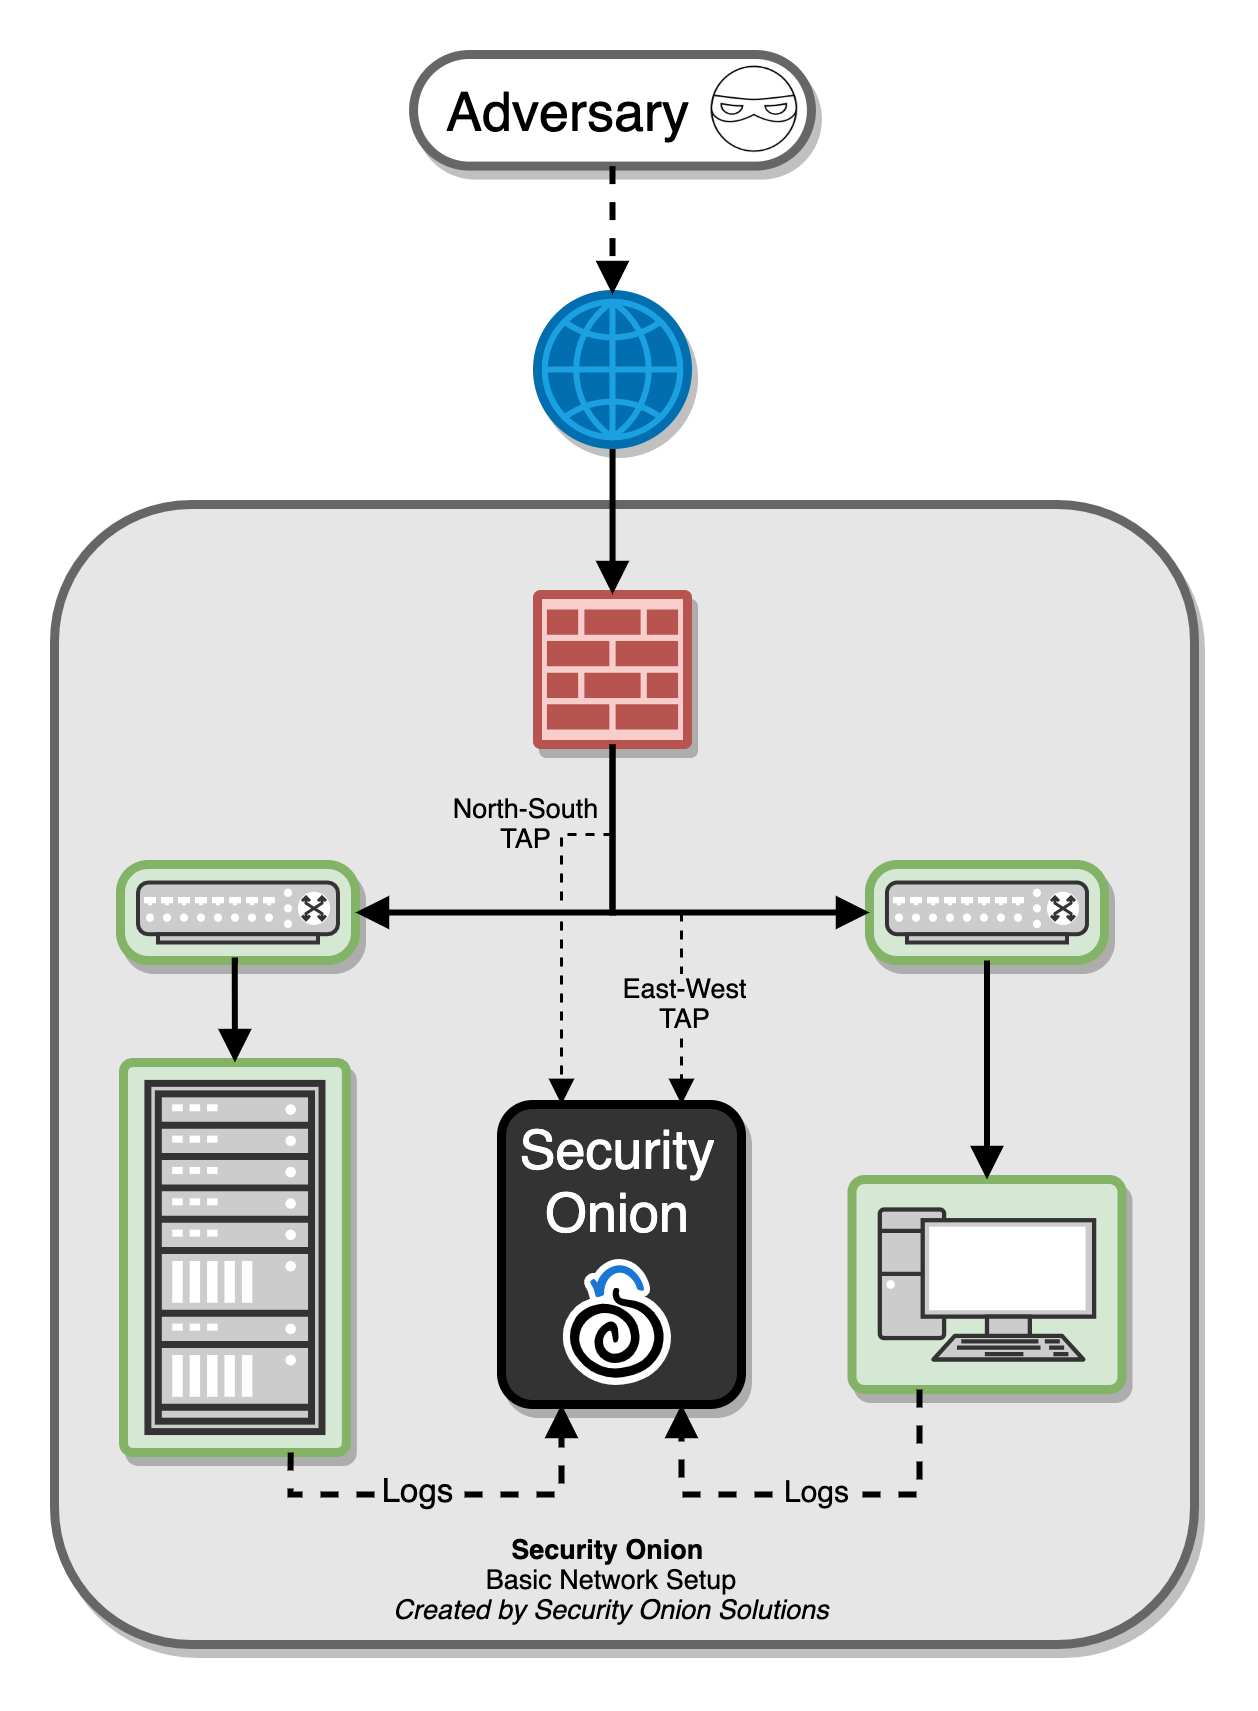
\includegraphics[width=8cm]{res/fig/SecOnionExample1.png}
    \caption{Esempio di utilizzo di Security Onion all'interno di un network enterprise \cite{SecOnionFig1}}
    \label{fig:seconionexample}
\end{figure}

Nella figura \ref{fig:seconionexample} si può vedere un esempio di utilizzo di Security Onion all'interno di un network enterprise.
In questo caso il traffico di rete viene duplicato ed inviato attraverso porte TAP a Security Onion che ne esegue l'analisi. Nel mentre anche i log dei sistemi monitorati vengono raccolti ed analizzati. In questo modo si hanno funzioni di NIDS e di HIDS.

Di seguito verranno brevemente descritti i principali software che vengono utilizzati all'interno di Secuirity Onion per poi analizzare l'architettura distribuita di tale IDS e il suo deploy all'interno dell'infrastruttura di testing.

\subsection{Tools integrati}
Di seguito verranno descritti i principali tools utilizzati da Security Onion durante il funzionamento all'interno di un'architettura distribuita. L'architettura in questione verrà meglio analizzata sucessivamente.
\subsubsection*{Suricata}
Suricata \cite{suricata} è un NIDS open source, maturo e robusto. Ispeziona il traffico di rete usando regole e linguaggio di signature oltre ad avere supporto a LUA \cite{LUA} scripting per rilevazione di minacce complesse. Attraverso l'integrazione di linguaggio di scripting è possibile, ad esempio, elaborare il payload di un pacchetto di rete prima di cercare possibili fingerprint match, aumentando le difese contro le tecniche di offuscamento. 
Suricata è anche in grado di agire attivamente in caso di intrusione, per questo motivo è anche classificato come Intrusion Prevention System (IPS). Inoltre é anche in grado di memorizzare PCAP files\footnote{file contenenti pacchetti catturati dal traffico di rete} per analisi successive.
Viene quindi principalmente usato come SIDS all'interno di Security Onion.
\subsubsection*{ZEEK}
ZEEK \cite{ZEEK} è un tool di analisi del traffico di rete. Al contrario di Suricata non è ottimizzato per la ricerca di signatures e non fornisce memorizzazione della cattura del traffico di rete. Il suo scopo è interpretare il traffico di rete e generare notevoli volumi di informazioni riguardanti il comportamento della rete, fornendo visibilità e contesto, oltre ad offrire capacità come:
\begin{itemize}
    \item Analisi della performance di rete;
    \item Profiling di host e servizi;
    \item Anomaly detection.
\end{itemize}
In Security Onion viene affiancato a Suricata per la rilevazione di minacce attraverso l'analisi del traffico di rete. Mentre Suricata permette di identificare attacchi basandosi sul signature matching, ZEEK permette di reperire il contesto dell'attacco,  offrendo tutti i metadata necessari per analizzare al meglio la situazione e poter quindi agire di conseguenza.

\subsubsection*{Stenographer}
Stenographer \cite{stenographer} è un utility per la cattura del traffico di rete cui scopo é memorizzare tutto il traffico catturato su disco per scopi di intrusion detection e incident response.
Fornisce un'implementazione ad alta performance della scrittura dei pacchetti da NIC a disco e gestisce la cancellazione automatica quando la memoria si satura. 
Offre inoltre metodi per la lettura rapida ed efficiente di set specifici di pacchetti oltre ad un linguaggio di query.

Si può accedere a cattura dei pacchetti memorizzai attraverso una qualsiasi interfaccia PCAP o attraverso Command Line Interface (CLI).

\subsubsection*{Strelka}
Strelka \cite{strelka} é un sistema di scansione di files in tempo reale, utilizzato per la ricerca e rilevazione di minacce o per analisi di incident response. Il suo scopo è l'estrazione di file e metadati su larga scala. È in grado di utilizzare regole YARA\footnote{le regole YARA usano pattern  come sequenze  di byte  o stringhe riconducibili  a malware noti } per l'identificazione di minacce note.

In Security Onion viene utilizzato per analizzare i file estratti da ZEEK e Suricata durante l'analisi del traffico di rete.

\subsubsection*{Sensoroni}
Sensoroni \cite{sensoroni} é un sistema software per il monitoraggio e l'interrogazione di server o dispositivi remoti.
È composto da un server e uno o più agenti.
Gli agenti sono  eseguiti sui dispositivi remoti (sensori) ed eseguono i \textit{jobs} che sono stati impartiti e accodati dal server. 
Il server offre un'interfaccia utente per gli amministratori per eseguire task come il monitoraggio dei sensori e la gestione dei jobs.

\subsubsection*{Elastic Stack}
Con Elastic Stack \cite{elasticstack} si intende una collezione di software open source appartenenti alla compagnia Elastic.
Il suo scopo è aiutare l'utente a raccogliere dati da qualsiasi sorgente e in qualsiasi formato per poter poi eseguire ricerche, analisi e visualizzazioni dei dati.
Questa collezione era precedentemente chiamata come ELK stack, dove ELK rappresenta l'acronimo delle sue componenti software, ovvero:
\begin{description}
    \item [Elasticsearch] Motore di ricerca e analisi distribuito, basato su interfaccia RESTful ed usato per moltissimi casi d'uso. Componente che rappresenta il cuore dell'Elastic Stack. Mantiene e indicizza i  dati per ricerche veloci e precise. 
    In Security Onion riceve i log e ne effettua il parsing prima di memorizzarli e indicizzarli.
    \item [Logstash] Motore di data processing server-side basato su pipeline, capace di raccogliere dati da moltitudine di sorgenti, trasformali ed inoltrarli.
    In Security Onion trasporta i log, su cui non è ancora stato effettuato parsing,  ad Elastic Search.
    \item [Kibana] Interfaccia GUI  che permette di visualizzare i dati memorizzati in Elastic Search e di navigare l'Elastic Stack. Permette di visualizzare in tempo reale flussi di dati di notevoli dimensioni e di aumentarne la comprensione attraverso grafici.
\end{description}

L'ELK stack si evolse nell'Elastic Stack in seguito all'aggiunta di Beats alla collezione.
Beats sono installati come agents su dispositivi remoti e vengono utilizzati per inviare dati di diversa natura (logs, metriche, dati di rete, etc.) direttamente a Elastic Search  o indirettamente attraverso Logstash. Security Onion in particolare usa FileBeat per inoltrare log a Elastic Search.

Lo stack viene principalmente usato per la gestione di ingenti quantità di dati o in caso siano necessarie capacità di ricerca avanzate sui dati. In Security Onion viene utilizzato per inoltrare, ricevere, memorizzare, indicizzare,visualizzare e analizzare i vari log generati.

\subsubsection*{ElastAlert}
ElastAlert \cite{elastalert} è un framework per l'allerta su anomalie, picchi  o altri pattern di interesse all'interno dei dati custoditi in Elasticsearch. Interroga Elasticsearch e fornisce un meccanismo di allerta in tempo reale con molteplici tipi di output. 

\subsubsection*{Curator}
Curator \cite{curator} è un Utility utilizzata all'interno di Elastic Stack per la gestione degli indici di Elasticsearch. In particolare: 
\begin{enumerate}
    \item Ottiene lista di indici da cluster, che verrà chiamata \textit{actionable};
    \item Itera su lista di filtri definiti da utente per rimuovere progressivamente indici dalla lista actionable;
    \item Esegue diverse azioni su elementi rimasti a seguito del filtraggio.
\end{enumerate}

\subsubsection*{Redis}
Redis \cite{redis} è uno store di strutture dati in memoria open source, utilizzato come database, cache e message broker. Supporta strutture dati come stringhe, hash, liste, insiemi, insiemi ordinati, etc.
I  dataset vengono mantenuti in memoria principale rendendo l'accesso estremamente veloce, ma i dati possono anche essere resi persistenti all'occorrenza.

Security Onion utlizza Redis come contenitore temporaneo dei log ricevuti da Logstash. I log così memorizzati vengono poi reperiti da Logstash e consegnati a Elastic Search.

\subsubsection*{Security Onion Console (SOC)}
SOC è l'interfaccia web attraverso cui un'analista può accedere ai vari tools di analisi offerti dalla piattaforma.
L'interfaccia web è divisa più sezioni.
Tra le sezioni built-in vi sono:
\begin{description}
    \item[Alerts] Visualizza gli \textit{alerts} che Security Onion sta generando. È possibile visualizzarne i dettagli e i PCAP a cui sono associati o aggiungere l'alert a dei Cases;
    \item[Dashboard] Permette di avere un overview generale del sistema. Personalizzabile all'occorrenza;
    \item[Hunt] Simile alla Dashboard ma più mirata alla ricerca di minacce;
    \item[Cases] Interfaccia per gestire i Cases. Attraverso i Cases é possibile raggruppare più alerts che si ritengono essere associati per studiare nel dettaglio la possibile intrusione o anomalia.
    \item[PCAP] Permette di analizzare i PCAP raccolti con Stenographer, anche in relazione ad un particolare evento;
    \item[Grid] Permette di controllare lo status dei nodi appartenenti al sistema Security Onion.
\end{description}

Oltre alle sezioni elencate vi sono collegamenti a tools che hanno interfacce web separate come Kibana, tra cui:
\begin{description}
    \item [Grafana ]  Permette di visualizzare attraverso grafici lo status e informazioni vitali del sistema come l'uso della CPU, RAM, traffico di rete, etc. \cite{grafana};
    \item [Playbook] Consente di creare una lista di strategie di rilevazione, dette \textit{Plays}. Ogni Play è composto di obiettivo, configurazione e \textit{follow-up}. L'obiettivo é l'oggetto da rilevare (eg. un'anomalia, un'intrusione) e necessita della configurazione necessaria per poter essere rilevato. Nel caso di Security Onion le configurazioni sono basate su ElastAlert. Con follow-up si intende le azioni da eseguire per validare e/o correggere quanto accaduto. 

    I risultati delle Play sono disponibili nelle sezioni Haunt, Dashboard e Kibana. Quando il risultato di una Play è di gravità elevata viene anche generato un alert visualizzabile nell'apposita sezione.
    Quando una Play viene attivata, la configurazione ElastAlert viene inserita in produzione.
    \item [ATT\&CK Navigator ] Il Navigator ATT\&CK è progettato per fornire una navigazione e un'annotazione di base delle tecniche appartenenti alla \textit{matrice MITRE ATT\&CK}\footnote{matrice standardizzata di tattiche e tecniche di minacce informatiche.} \cite{att&ck}. Può essere utilizzato  per visualizzare la  copertura difensiva, la pianificazione del  team di attacco/difesa, la frequenza delle tecniche rilevate e molto altro.
    Inoltre si integra con Playbook, permettendo di visualizzare le Plays in relazione alle tecniche coperte nella matrice ATT\&CK per avere un'idea ancora più chiara della copertura difensiva \cite{att&ckNavigator}.
\end{description}

\subsubsection*{Host-based visibility tools}
Security Onion permette anche la raccolta di molti tipi di log generati dagli host che si desiderano monitorare. L'host può scegliere tra diverse tecnologie agent-based per effettuare diversi task di controllo sull'host ed inviare i relativi logs a Security Onion.

Attraverso specifiche tecnologie installate sugli host da monitorare e l'analisi dei relativi log è possibile implementare il lato HIDS di Security Onion già accennato in precedenza.
In alternativa, si potrebbe decidere di inviare logs arbitrari usando una delle seguenti tecnologie:
\begin{description}
    \item[Osquery] Osquery \cite{osquery} è un agent  capace di astrarre l'host, sul quale è installato, a database relazionale. L'agent può quindi essere interrogato usando sintassi SQL per avere informazioni sul sistema. Questo può anche essere usato inviare i log a Security Onion.
    \item[Wazuh] Wazuh \cite{wazuh} è un agent con capacità di HIDS. Verrà approfondito meglio nella sezione inerente gli agents. Permette anche l'inoltro di logs a Security Onion.
    \item[FileBeat] Come già spiegato precedentemente, FileBeat \cite{filebeat} è in grado di fornire trasporto di log dedicato.
    \item [Syslog] Syslog \cite{syslog} è un protocollo di rete usato per l'invio di log semplici. Utile nel caso non sia possibile installare un agent sull'end-point.
\end{description}

\subsection{Architettura}
Security Onion dispone di diverse Architetture possibili per adattarsi alle diverse esigenze e risorse, tuttavia l'architettura raccomandata è quella distribuita che verrà di seguito analizzata.

L'architettura distribuita offre maggior scalabilità e una maggior performance in quanto basta aggiungere nodi per poter maneggiare più traffico di rete o sorgenti di logs.

Si compone di  tre tipologie di nodi:
\begin{itemize}
    \item Forward Node;
    \item Manager Node;
    \item Search Node.
\end{itemize}

\vspace{5mm}
Il Forward Node è un sensore che esegue Zeek, Suricata, Stenographer e Wazuh per generare logs. In particolare, come detto, Zeek e Suricata analizzano il traffico di rete, Wazuh funge da HIDS sull'end-point e Stenographer memorizza i PCAP all'interno di esso. Tutti i logs vengono inviati attraverso FileBeat a Manager Node. I PCAP vengono all'occorrenza reperiti dal Forward Node attraverso il Sensoroni agent.
Strelka analizza all'occorrenza i file estratti da Zeek.

\vspace{5mm}
Il Manager node riceve attraverso Logstash i logs  inviati dai sensori e li mette in coda su Redis.
Hanno anche un'istanza di Elasticsearch che viene usata per memorizzare i Cases e le configurazioni centrali oltre ad effettuare le query sulle istanze ElasticSearch dei Search Nodes.
Esegue inoltre:
\begin{itemize}
    \item Security Onion Console per permettere ad un'analista di interfacciarsi con esso;
    \item Kibana per visualizzare  i logs indicizzati con Elasticsearch;
    \item Curator per gestire gli indici ed eseguire operazioni su essi;
    \item ElastAlert per generare alerts  in Elasticsearch;
    \item Wazuh come istanza HIDS locale;
\end{itemize}
Attraverso il Manager Node l'analista può interfacciarsi con Security Onion per eseguire query e reperire/analizzare dati.

\vspace{5mm}
Il Search Node usa Logstash per consumare logs da coda in Manager Node per poi eseguirne il parsing e l'indicizzazione con ElasticSearch. Usa Curator per gestire gli indici e ha Wazuh installato come agent HIDS. Quando analista esegue queries su Manager Node, questo esegue a sua volta queries su Search Nodes e ne restituisce il risultato.
L'aggiunta di Search Nodes può avvenire attraverso \textit{cross cluster search}, dove ogni Search Node è indipendente, o attraverso \textit{clustering} tradizionale in cui tutti i Search Nodes si uniscono logicamente per formare un singolo cluster.

\subsection{Deploy e requisiti Hardware}
In questa sezione verrà inizialmente descritto in che modo i vari nodi dell'infrastruttura utilizzano le risorse di calcolo, per poi passare all'elenco dei requisiti minimi di sistema \cite{securityOnionRequirements} dei singoli nodi e l'effettivo dispiegamento delle risorse invece utilizzato sulle macchine virtuali.
Le risorse sono state calcolate considerando 1 Gbps come massimo carico di rete.
In conclusione seguirà una breve analisi del  deploy dell'IDS all'interno dell'infrastruttura di testing.


\subsubsection*{Manager Node}
Il Manager Node utilizza la CPU principalmente per ricevere i logs in ingresso e posizionarli in coda su Redis, eseguire web server e aggregare i risultati ottenuti dai vari Search Nodes in seguito a querie. 

Le risorse della RAM vengono usate in particolare da esecuzione di Logstash e Redis. Le dimensioni della RAM impattano direttamente sulla dimensione della coda Redis.

La memoria secondaria invece  per utilizzi generali di sistema operativo e per mantenere la Dashboard di Kibana.


\begin{table}[hbtp]
    \centering
    \begin{tabular}{|l|c|c|c|}
        \hline
        & CPU (cores) & RAM (GB) & DISK (GB) \\
        \hline
        Minimi     & 4-8 & 16 & 200-1000   \\
        \hline
        Utilizzati & 8   & 16  & 200 \\
        \hline
    \end{tabular}
    \caption{Requisiti minimi e risorse effettivamente assegnate al Manager Node}
    \label{tab:requisitiHw1}
\end{table}


\subsubsection*{Search Node}

Search Nodes usano la CPU principalmente per eseguire il parsing e l'indicizzazione dei log, ovviamente la richiesta di CPU aumenta all'aumentare del numero di log da elaborare.

La quantità di RAM a disposizione influenza direttamente la velocità di ricerca all'interno degli indici e l'affidabilità del sistema di ricerca. I Programmi principalmente coinvolti nell'utilizzo della RAM sono Logstash ed Elasticsearch.

La memoria secondaria viene utilizzata per memorizzare metadati indicizzati. All'aumentare dello spazio a disposizione è possibile aumentare i tempi di conservazione dei dati.

\begin{table}[hbtp]
    \centering
    \begin{tabular}{|l|c|c|c|}
        \hline
        & CPU (cores) & RAM (GB) & DISK (GB) \\
        \hline
        Minimi     & 4-8 & 16-64 & >200   \\
        \hline
        Utilizzati & 8   & 16  & 200 \\
        \hline
    \end{tabular}
    \caption{Requisiti minimi e risorse effettivamente assegnate al Search Node}
    \label{tab:requisitiHw2}
\end{table}



\subsubsection*{Forward Node}
La CPU di un Forward Node viene utilizzata per analizzare e memorizzare il traffico di rete. All'aumentare del traffico di rete aumenta il consumo del tempo di CPU necessario per l'analisi dei dati. 

Si stima che un worker Suricata o Zeek possa elaborare 200 Mbps, ciò implica che per gestire 1 Gbps di traffico di rete siano necessari almeno 10 worker e quindi almeno 10 cores. A questi vanno aggiunti i cores necessari per eseguire altri processi fondamentali come Stenographer, etc.

La RAM impiegata dipende molto dai servizi attivi, dal tipo di traffico monitorato, dal traffico attuale e dall'ammontare di pacchetti scartati che si considera accettabile. Viene principalmente utilizzata per scrivere cache e processare il traffico di rete.

La memoria secondara dipende da quanti dati si vogliono mantenere memorizzati per analisi future e dal periodo di retention\footnote{specifica dopo quanto tempo i dati verranno cancellati} ritenuto opportuno.
Se ad esempio si volesse mantenere il traffico di rete di un'intera giornata di monitoraggio, supponendo che il traffico di rete ricevuto abbia una media di 1 Gbps, allora serebbero necessari circa 11 TB di spazio di archiviazione solo per mantenere i PCAP.

\begin{table}[hbtp]
    \centering
    \begin{tabular}{|l|c|c|c|}
        \hline
        & CPU (cores) & RAM (GB) & DISK (GB) \\
        \hline
        Minimi     & $\approx 12$ & 16-128 & variabile   \\
        \hline
        Utilizzati & 13   & 64  & 500 \\
        \hline
    \end{tabular}
    \caption{Requisiti minimi e risorse effettivamente assegnate al Forward Node}
    \label{tab:requisitiHw3}
\end{table}


\vspace{7mm}
\subsubsection*{Deploy}
Il primo passo di deploy dell'IDS all'interno dell'infrastruttura di testing è stato creare una VM all'interno del server ESXi ed installarci sopra il Manager Node. Il Manager Node ha un'interfaccia di rete collegata alla Vlan con accesso ad Internet.

In seguito è stato installato il Search Node all'interno di un'altra VM. Questa ha una sola interfaccia di rete collegata alla stessa Vlan del Manager Node. Il nodo di ricerca è stato quindi collegato al Manager.

Infine è stata creata un'ulteriore VM in cui è stato installato il Forward Node. Questa ha due interfacce di rete. Una collegata alla stessa rete del Manager Node, mentre l'altra è collegata alla Botnet Vlan di cui si vuole monitorare il traffico di rete. In particolare quest'ultima deve essere in modalità promiscua\footnote{in modalità promiscua l'interfaccia di rete lascia passare anche il traffico non rivolto all'interfaccia stessa, verso la cpu}.
In una situazione normale sarebbe necessario duplicare il traffico di rete attraverso TAP o SPAN ed inviarne una copia all'interfaccia del Forward Node per poterlo analizzare, ma in questo caso particolare non è necessario. Infatti grazie al network virtualizzato del server ESXi basta impostare il virtual switch in modalità promiscua e tutto il traffico di rete sarà catturabile.

Una volta terminata l'installazione sono state aggiunte regole al Firewall integrato di Security Onion per poter accedere all'interfaccia web del Manager Node. 
Una volta impostato l'indirizzo di rete da monitorare è stato accertato che i servizi funzionassero correttaente.
In particolare sono state attivate tutte le regole built-in di Suricata e sono stati effettuati dei semplici test di scansione con Nmap\footnote{software utilizzato per eseguire scansioni di rete} \cite{nmap}  per verifica che le scansioni venissero effettivamente  rilevate.

%sistemare grafica e aggiungere tabelle con requisiti minimi e adoperati per ogni nodo.


\subsection{SALT}


Salt \cite{salt} è il componente principale di Security Onion incaricato del management di tutti gli altri nodi del sistema  IDS.

Salt è un framework per l'automazione cui funzionalità principali sono:
\begin{itemize}
    \item Capacità di gestire configurazioni di nodi da remoto;
    \item Esecuzione di comandi  e prelievo di dati su nodi remoti.
\end{itemize}

Oltre a queste capacità offre comunque tantissime altre funzionalità come Job Management, Job Scheduling, File Server, orchestration, etc.


In particolare la funzionalità di Configuration Management offerta permette di centralizzare le configurazioni di tutti i nodi dell'infrastruttura, oltre ad astrarre l'infrastruttura ad un insieme di dati.

Basato su architettura Master-Minions, dove master controlla uno o più minions. Comandi sono generati da master verso gruppo di minions, che eseguono tasks e ne ritornano i risultati/dati a master.

I messaggi tra Master e Minions avvengono attraverso \textit{ZeroMQ message bus} \cite{zeromq}. La comunicazione tra Master e Minion è criptata, utilizzando crittografia a chiave pubblica per l'autenticazione del Minion e  crittografia a chiave privata per scampio di dati.

Salt è basato su agents installati sui  minions ma è anche possibile gestire i nodi attraverso SSH senza dover installare necessariamente un agent apposito (agent-less system).

Il framework è scritto in Python ma il sistema di management delle configurazioni è di fatto lenguage-agnostic, ovvero aperto a qualsiasi tipo di linguaggio.
Di default usa YAML\footnote{linguaggio per serializzazione di dati in maniera comprensibile all'utente, utilizzato spesso per file di configurazione}   \cite{yaml} e Jinja\footnote{template engine} \cite{jinja} templates per le configurazioni.

Tra le features offerte da Salt vi sono anche:
\begin{description}
    \item[Fault tollerance]  Minion può connettersi a molteplici masters contemportaneamente;
    \item[Configuration Management scalabile] Il Design realizzato permette il management di migliaia di nodi;
    \item[Parallel execution] Comandi eseguibili in parallelo;
    \item[Python API] Interfaccia di programmazione semplice con design modulare ed estendibile.
\end{description}



\subsubsection{Remote execution}
Come accennato Salt usa modello master-client in cui master inoltra comandi a client che provvede ad eseguirli.

Entrando nel dettaglio, il Salt Master é un server che esegue un particolare processo chiamato \textit{salt-master}.  Inoltra comandi a  servers (Salt Minions) registrati presso il master che eseguono processo chiamato \textit{salt-minion}.

Salt può anche essere visto come un modello \textit{publisher-subscriber}. Il Master pubblica \textit{jobs} che devono essere eseguiti e Minions si iscrivono a questi jobs.

Quando un Minion termina l'esecuzione di un job, invia dati in risposta al Master. Salt usa due porte in particolare su ogni nodo per le comunicazioni tra master e minion.  Queste porte lavorano in contemporanea per ricevere e inviare dati verso il message bus.
Il Message Bus usa ZeroMQ per creare una topologia di rete asincrona per la comunicazione più veloce possibile.
In particolare usa due canali:
\begin{description}
    \item [Pub Channel] Canale usato da master per inviare jobs a minions. Basato su paradigma pub/sub.
    \item [Req Channel] Canale usato da minions per inviare dati a master. Usato principalmente per eseguire \textit{fetch} di files e inviare risultati di jobs.
\end{description}


La sintassi di un comando eseguibile da remoto verso uno  o più minions é della seguente forma:

\begin{center}
\begin{BVerbatim}
salt '<target>' <module>.<function> [arguments]
\end{BVerbatim}
\end{center}
\subsubsection{Configuration Management}
Il Configuration Management è eseguito dichiarando in quale stato dovrebbe essere un minion specifico, questo stato è chiamato Salt State. Questi altro non sono che file YAML, attraveso i quali è possibile eseguire il management dell'infrastruttura.
Un esempio di semplice Salt State:
    \begin{Verbatim}[numbers=left,frame=single,fontsize=\small]
        install_network_packages:
            pkg.installed:
                - pkgs:
                    - rsync
                    - lftp
                    - curl
    \end{Verbatim}
L'esempio  mostra un Salt State usato per installare o mantenere l'installazione di alcuni pacchetti. I file Salt State hanno estensione \textit{.sls}.

Per portare manualmente un minion specifico in questo stato si può usare il comando:
\begin{center}
    \begin{BVerbatim}
salt "<nome minion>" state.apply <Salt State> 
    \end{BVerbatim}
\end{center}

Ovviamente non è pensabile eseguire il precedente comando manualmente per portare ogni minion in un determinato stato, soprattutto per ambienti in cui vi sono migliaia di minions con migliaia di State files. Per questo motivo viene usato il \textit{Top File}.

Il Top File é uno State File usato per  mappare i Salt States ai vari minions. In breve, esso descrive dove determinati Salt States devono essere applicati.
Un esempio di Top File è il seguente:
    \begin{Verbatim}[numbers=left,frame=single,fontsize=\small]
        base:
          '*':
             - common
          'minion1':
              - sample
    \end{Verbatim} 
Questo Top File associa il Salt State \textit{common.sls} a ogni minion e \textit{sample.sml} al minion \textit{minion1}
Attraverso il comando che segue é possibile applicare il Top File a tutti i minions:
\begin{center}
    \begin{BVerbatim}
salt * state.highstate
    \end{BVerbatim}
\end{center}

I Salt State possono essere parametrizzati attraverso l'uso di  \textit{pillars} e meccanismi di template.
I pillars sono file in master che contengono dati che devono essere distribuiti a minions. Questi dati possono essere ad esempio dati sensibili, password, configurazioni, chiavi crittografiche, e molto altro.
I pillars sono associati ai vari Minions con un apposito \textit{Top File} dedicato, in modo analogo a quanto avviene con i Salt States.
Un esempio di pillar contenenti id di utenti:
    \begin{Verbatim}[numbers=left,frame=single,fontsize=\small]
        users:
          thatch: 1000
          shouse: 1001
          utahdave: 1002
          redbeard: 1003
    \end{Verbatim}

I dati dei pillars possono essere referenziati all'interno dei Salt State usando dei template, come ad esempio il seguente Salt State:
    \begin{Verbatim}[numbers=left,frame=single,fontsize=\small]
        
        {{user}}:
          user.present:
            - uid: {{uid}}
        
    \end{Verbatim}
Questo State usa la sintassi di template Jinja per creare una logica più complessa, in particolare prende i dati contenuti all'interno del pillar precedentemente definito per assicurarsi che all'interno del minion, a cui verrà applicato lo State, siano presenti gli user id elencati nel pillar.
%qui spiega benissimo:
%https://docs.saltproject.io/en/latest/topics/development/architecture.html 
%https://docs.saltproject.io/salt/user-guide/en/latest/topics/execution-architecture.html

\subsubsection{Salt in Security Onion}
Come già detto Salt è usato all'interno di Security Onion per il management di tutti i nodi all'interno dell'infrastruttura.

Molte delle opzioni di Security Onion sono configurabili attraverso specifici pillar files.

Modificando i pillars è possibile cambiare le configurazioni di tools. Tra i tools che è possibile modificare attraverso le impostazioni nei Pillars vi sono: Filebeat, Suricata, Zeek, Managing Alerts, etc.


Oltre al mantenere le configurazioni per i vari software, attraverso Salt è anche possibile eseguire comandi sui nodi e controllarne lo stato, permettendo controllo totale sull'infrastruttura Security Onion.


\section{Ossim}
Ossim \cite{ossim} è un prodotto Security Information and Event Management (SIEM)  open source sviluppato da AT\&T Cybersecurity (in passato denominata AlienVault). Un sistema SIEM colleziona dati attingendo da diverse fonti di logs all'interno dell'infrastruttura. 
Attraverso l'analisi dei dati è capace di generare allarmi in caso di eventi sospetti, oltre a poter generare reports.
Ossim viene integrato con Open Threat Exchange (OTX), una piattaforma in cui utenti possono scambiarsi informazioni su host maligni.

È in grado di supportare logs di diversa natura e da molteplici sorgenti. È anche possibile inoltrare coppia di traffico di rete.

Ossim è costituito di tre elementi:
\begin{description}
    \item [Sensore] Primo device ad avere un contatto con i logs. Raccoglie logs ed informazioni che riceve e lì converte in eventi per poi inviarli a Server.
    \item [Server] Processa eventi ricevuti da sensore ed esegue operazioni come correlazione di eventi, pattern recognition e calcolo del rischio. Inoltre esegue anche controlli sfruttando informazioni di OTX.
    \item [Logger] Nodo sul quale vengono memorizzati i logs. Comprime, firma e memorizza informazioni in accordo alle retention policies.
\end{description}

Ossim è incentrato sul concetto di Asset. Un Asset è un qualsiasi elemento dotato di indirizzo IP.
Ogni Asset aggiunto deve passare attraverso i seguenti moduli per poter avere il massimo livello di accuratezza di output da Ossim:
\begin{description}
    \item [Asset Discovery] Modulo che identifica assets e porte note. Cerca inoltre di mantenere un inventario degli Assets identificati.
    \item [Vulnerability Assessment] Identifica vulneravilità in Assets attraverso scansioni. Le scansioni possono essere più approfondite attraverso autenticazione.
    \item [Intrusion Detection] Costituito da NIDS, HIDS e File Integrity Monitor (FIM). Utilizza tools come Snort per identificare intrusioni in  traffico di rete in generale e Suricata per intrusioni su traffico web-based. 
    \item [Behavioral Monitoring] Modulo in cui vengono analizzate le anomalie di rete. Utilizza modulo Netflow per identificare cause di spikes di rete, propagazione di malware, etc.
    Possiede anche capacità di monitoraggio dell'availability di host e servizi.
    \item [Security Intelligence] Modulo in cui processamento/computazione di eventi è eseguito. Tutte le info prese da moduli precedenti vengono analizzate al suo interno per creare reports. 
\end{description}

Ossim e l'intera infrastruttura è configurabile e gestibile una volta installato attraverso l'interfaccia web.


\subsection*{Dopley e requisiti Hardware}

Ossim è stato utilizzato come IDS da affiancare a Security Onion. È stato utilizzato principalmente per potrer confrontare i risultati di Security Onion con un secondo IDS e per approfondire un sistema  IDS alternativo.

Per semplicità ne è stato eseguito il deploy in formato stand-alone, ovvero con tutti e tre gli elementi che lo compongono in stesso host.

La macchina virtuale sul quale è stato installato OSSIM ha due interfacce di rete: \begin{itemize}
    \item  NIC di management collegata alla Vlan con accesso ad Internet per potersi interfacciare con la web gui.
    \item  NIC collegata alla Botnet Vlan in modalità promiscua, necessaria per sniffare il traffico di rete.
\end{itemize} 

I requisiti Hardware richiesti  e soddisfati per gestire dai 1000 ai 2000  eventi al secondo sono i seguenti:
\begin{table}[hbtp]
    \centering
    \begin{tabular}{|l|c|c|c|}
        \hline
        & CPU (cores) & RAM (GB) & DISK (GB) \\
        \hline
        Minimi     & 8 & 16-24 & 500-1000   \\
        \hline
        Utilizzati &  8  & 24 & 500 \\
        \hline
    \end{tabular}
    \caption{Requisiti minimi e risorse effettivamente assegnate ad Ossim}
    \label{tab:requisitiHw4}
\end{table}

\chapter{Studio Botnet 1 - Byob}
%descrizione OK
%funzionamento ad alto livello OK
%funzionamento a basso livello
%deploy (docker), note debug e modifiche
%rilevamento con ids
    

Byob \cite{byob} é una Botnet open source scritta in Python, creata appositamente per scopi educativi e di testing.
Si compone di quattro categorie di moduli principali:
\begin{itemize}
    \item Server Module
    \item Client Module
    \item Post-exploitation Modules
    \item Core Modules
\end{itemize}

I moduli Core racchiudono le funzionalità principali di Byob e sono utilizzate all'interno del Client Module e del Server Module.  

Il modulo Server viene utilizzato per inizializzare il C\&C Server. Utilizza Flask \cite{flask} come framework e  dispone di un database Sqlite \cite{sqlite} per mantenere i dati e le sessioni dei bot anche a distanza di tempo e in presenza di disconnessioni. Offre controllo sui bot attraverso console collegata via \textit{reverse-shell}\footnote{shell remota a cui viene reindirizzato input e output verso host che vuole accedervi} o attraverso interfaccia web dedicata. Basato su topologia centralizzata con paradigma push-based (il server invia i comandi ai bot).

Il modulo Client è utilizzato per creare i payloads che verranno utilizzato per generare i bot. In particolare il payload è un multi-stage installer che verrà analizzato meglio nel dettaglio.  Il bot così generato sarà in grado di importare moduli necessari e arbitrari direttamente dal server e di caricarli in memoria, non lasciando così traccie su disco. Questo meccanismo permette al bot di non avere dipendenze pregresse se non avere Python installato. Tuttavia per ovviare anche a questa dipendenza è possibile creare eseguibili che includano all'interno, oltre al payload, un interprete Python stand-alone, così che neanche Python risulti più una dipendenza.  Il payload può anche essere opzionalmente criptato e opzionalmente può abortire l'esecuzione se rileva che il sistema sul quale sta eseguendo é una macchina virtuale.

I moduli post-exploitation sono moduli built-in che possono essere importati ed eseguiti su bot e offrono funzionalità operative molto interessanti.
Tra questi possiamo trovare:

\begin{description}
    \item [Persistence] Cerca di rendere il malware persistente all'interno del sistema che lo ospita;
    \item [Packet Sniffer] Cattura traffico di rete;
    \item [Escalete Privileges] Tenta di ottenere privilegi di amministratore;
    \item [Port Scanner] Scansiona traffico di rete;
    \item [Keylogger] Cattura digitazioni della tastiera;
    \item [Screenshot] Cattura immagine del monitor;
    \item [Outlook] Utilizza Outlook client per leggere/scrivere email;
    \item [Process Control] Per elenacare/ricercare/terminare processi;
    \item [iCloud] Cerca account autenticati ad iCLoud su macOS
    \item [Miner] Utilizza miner per minare criptovaluta;
\end{description}

Oltre a questi moduli built-in, il bot può anche importare moduli creati ad-hoc dal botmaster.




\begin{figure}[hbtp]
    \centering
    \begin{subfigure}[hbtp]{0.45\textwidth}
        \centering
        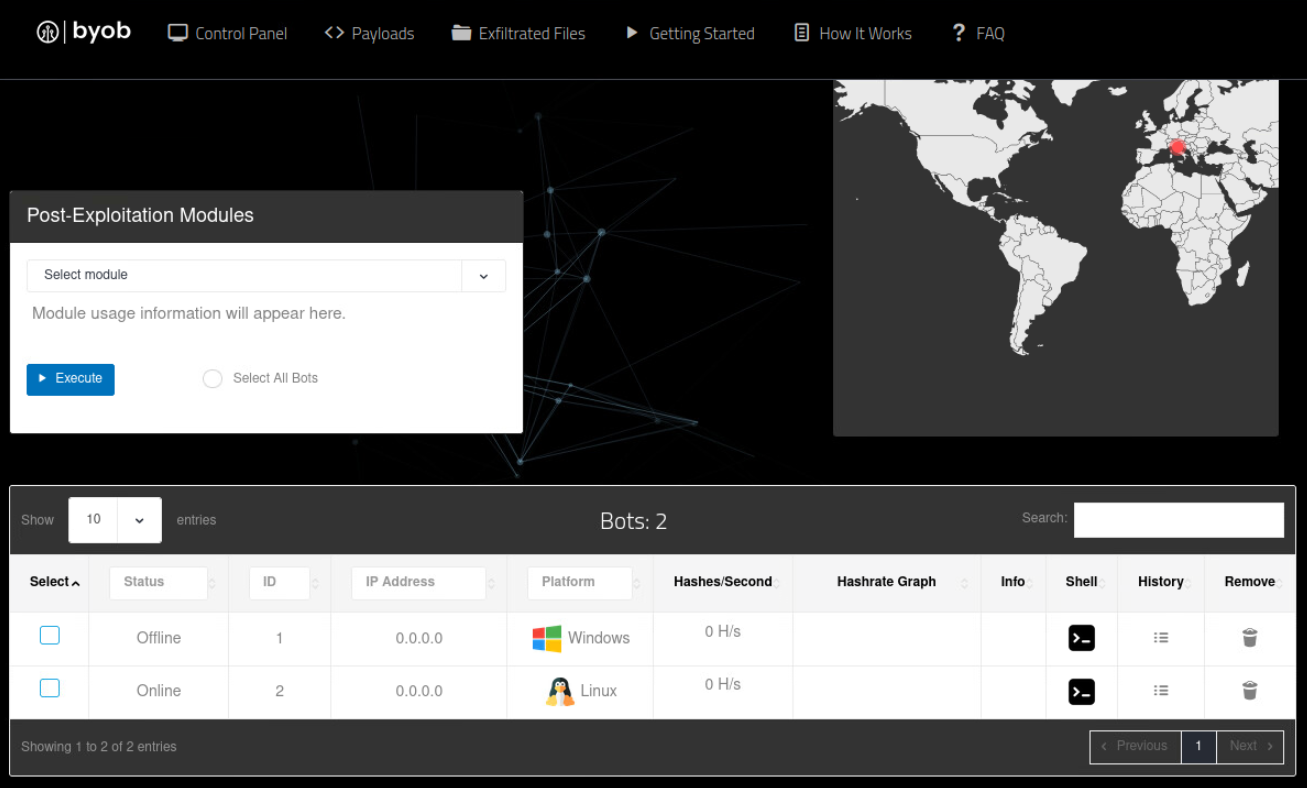
\includegraphics[width=\textwidth, height=6cm]{res/fig/byob-home.png}
        \caption{}
        \label{fig:byobhome}
    \end{subfigure}
    \hfill
    \begin{subfigure}[hbtp]{0.45\textwidth}
        \centering
        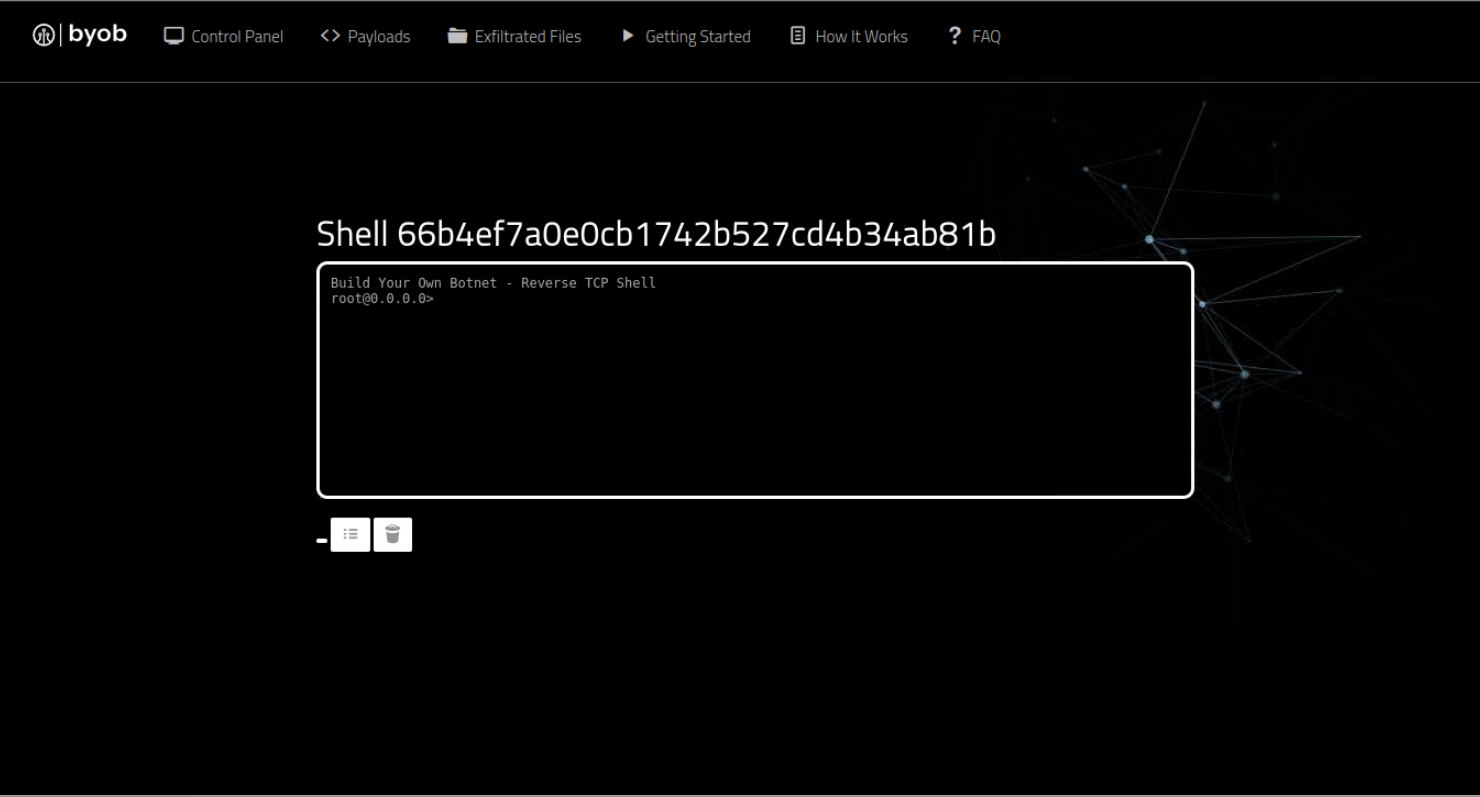
\includegraphics[width=\textwidth , height=6cm]{res/fig/byob-shell.png}
        \caption{}
        \label{fig:byobshell}
    \end{subfigure}
    \caption{(a) Home page; (b) Pagina shell;}
    \label{ciao1}
\end{figure}

Nella \Cref{fig:byobhome}  si può vedere la schermata di controllo principale dell'interfaccia web di Byob. In basso è presente una schermata con i bot attualmente collegati. Sul lato sinitro sinistro vi è  un pannello con i moduli di post-exploitation utilizzabili sui bot del pannello sottostante, mentre a destra si può controllare la posizione geografica del bot. 

Cliccando sull'icona del terminale in corrispondenza di un bot nel pannello inferiore, reindirizza il browser verso una schermata in cui viene emulato un terminale. Questo è collegato al bot attraverso reverse-shell e può essere usato per operare direttamente sul bot.
\begin{figure}[hbtp]
    \centering
    \begin{subfigure}{0.45\textwidth}
        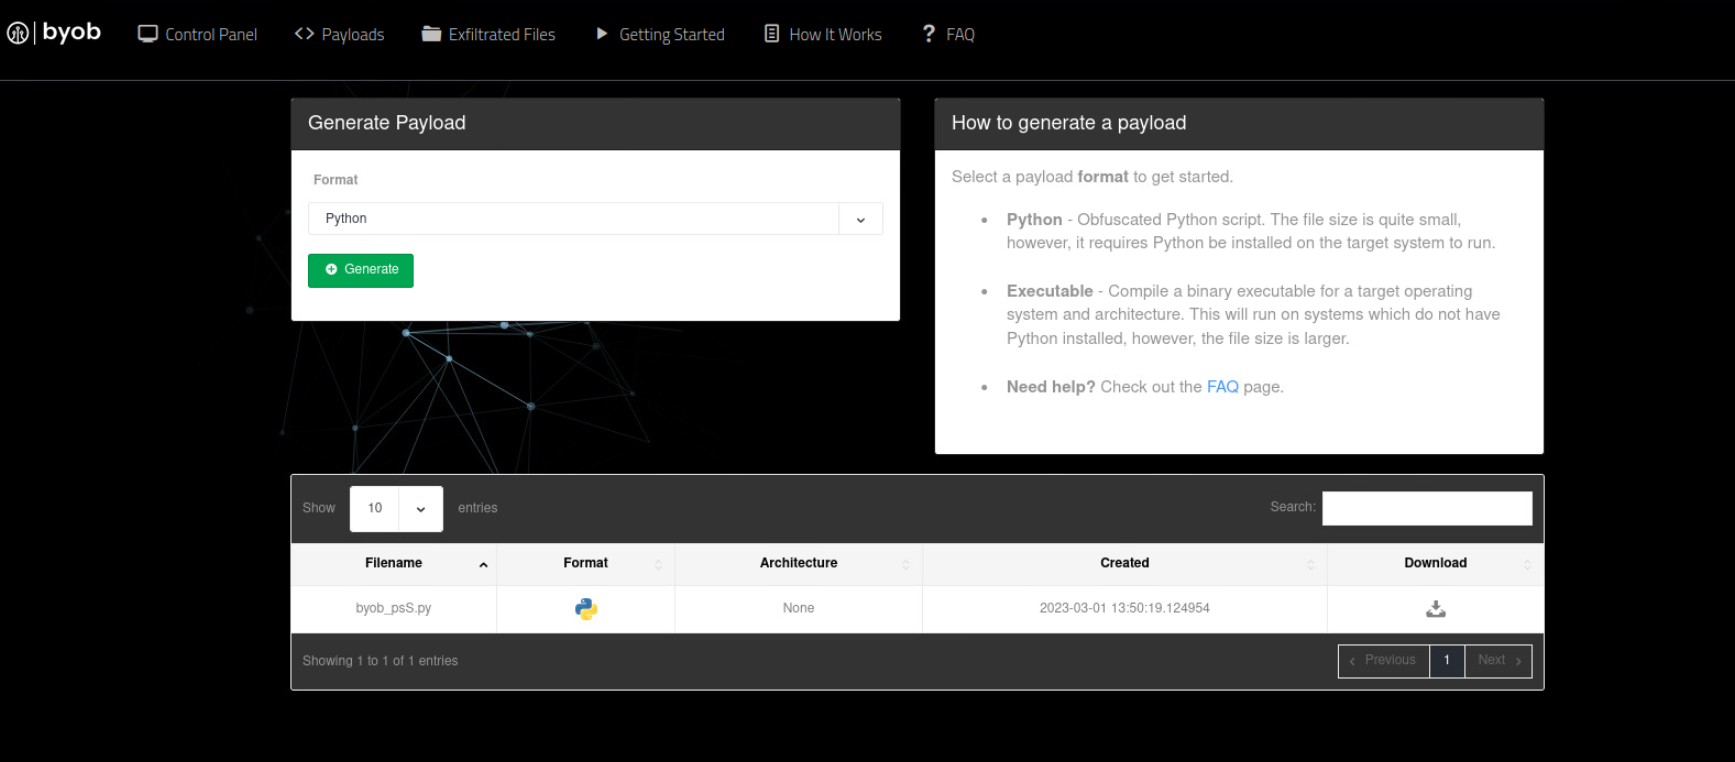
\includegraphics[width=\textwidth , height=6cm]{res/fig/byob-payloads.png}
        \caption{}
        \label{fig:byobpayloads}
    \end{subfigure}
    \hfill
    \begin{subfigure}{0.45\textwidth}
        \centering
        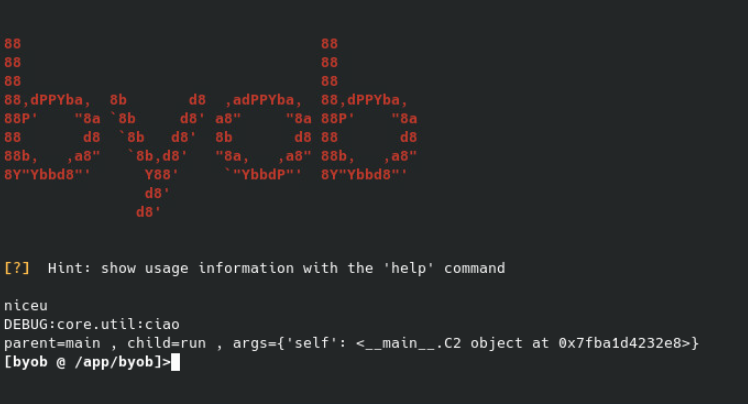
\includegraphics[width=\textwidth , height=6cm]{res/fig/byob-console.png}
        \caption{}
        \label{fig:byobconsole}
    \end{subfigure}
    \caption{(a) Schermata di generazione dei payloads; (b) Byob console.}
    \label{ciao2}
\end{figure}

In \Cref{fig:byobpayloads} si può esservare la schermata di creazioned dei payloads. I payload possono essere eseguibili compilati o script Python. Una volta creati possono essere scaricati da questa pagina web.

Byob può essere anche eseguito nella sua variante minimale da console ( \Cref{fig:byobconsole}).


Attraverso il pannello di controllo o le console è possibile controllare i bot ed eseguire le classiche funzionalità RAT o eseguire moduli python arbitrari, rendendo di fatto possibile eseguire qualsiasi operazione\footnote{per alcune operazioni può essere necessaria l'autenticazione come amministratore} sulle macchine vittime.


\section{Dettagli implementativi}
Nella seguente sezione verranno descritti più nel dettaglio i principali componenti su cui è basata la Botnet.

\subsection{Server}
Lo script \textit{Server.py} è il responsabile dell'esecuzione del server e di tutte le sue funzionalità. In \Cref{fig:byobumlserver} si può vedere un diagramma di sequenza che ne descrive il comportamento.

Al momento dell'esecuzione crea tre sottoprocessi che eseguiranno in background:
\begin{description}
    \item[Packages handler] Mantiene un server HTTP su porta dedicata incaricato di fornire Python Packages richiesti da bot.
    \item[Module handler] Mantiene un server HTTP su porta dedicata incaricato di fornire Moduli Python richiesti da bot.
    \item[Request handler] Gestisce le richieste POST di upload  inviate da bot, salvando i file in apposite directory.
\end{description}
Sucessivamente, esegue il C\&C server su un'altra porta dedicata.
Il C\&C server crea un thread che si occupa di gestire le nuove connessioni inizializzate dai bot. Per ogni nuovo bot connesso crea una sessione, cui informazioni vengono salvate in database ed aggiornate ad ogni connessione. 

Una volta creato il thread, si occupa di gestire i comandi inseriti su console di controllo dei bot e le richieste  dell'interfaccia web.
Come già osservato nell'introduzione di questo capitolo, Byob può eseguire anche senza interfaccia web e in tal caso la console non è inizialmente collegata ad un bot. La console emulata dell'interfaccia web, invece, è già associata al bot specifico. 

Quando byob esegue in console, ha a disposizione dei comandi, di cui la versione con interfaccia web non ha bisogno, dato che sono integrati all'interno delle pagine web (eg. controllare le sessioni attive).

Durante il ciclo di vita del C\&C, la console  rimane in attesa di input. Quando viene inserito un comando,  ne effettua il parsing per controllare che sia un comando disponibile e nel caso lo esegue con eventuali parametri annessi.
 Una volta collegata alla sessione del bot, questa rimane in attesa di comandi da inoltrare. 
 La versione web usa uno script Javascript per inviare una richiesta POST contenenti i comandi digitati al backend che si occupa di inoltrarlo al bot.
 La versione console invece crea un thread che è incaricato di inviare i comandi direttamente al bot, e li inoltra solo in risposta a richieste di polling da parte del bot.
 Si può quindi affermare che la versione web sia push-based mentre l'altra pull-based.
 
 Da questo punto in avanti le funzionalità di console e  console web emulata sono identiche, la versione web infatti sfrutta le funzionalità riadattate di Byob versione console.

Il server invia comandi e riceve risultati sotto forma di dizionari contenenti altre informazioni come l'id del bot.


\begin{figure}
    \centering
    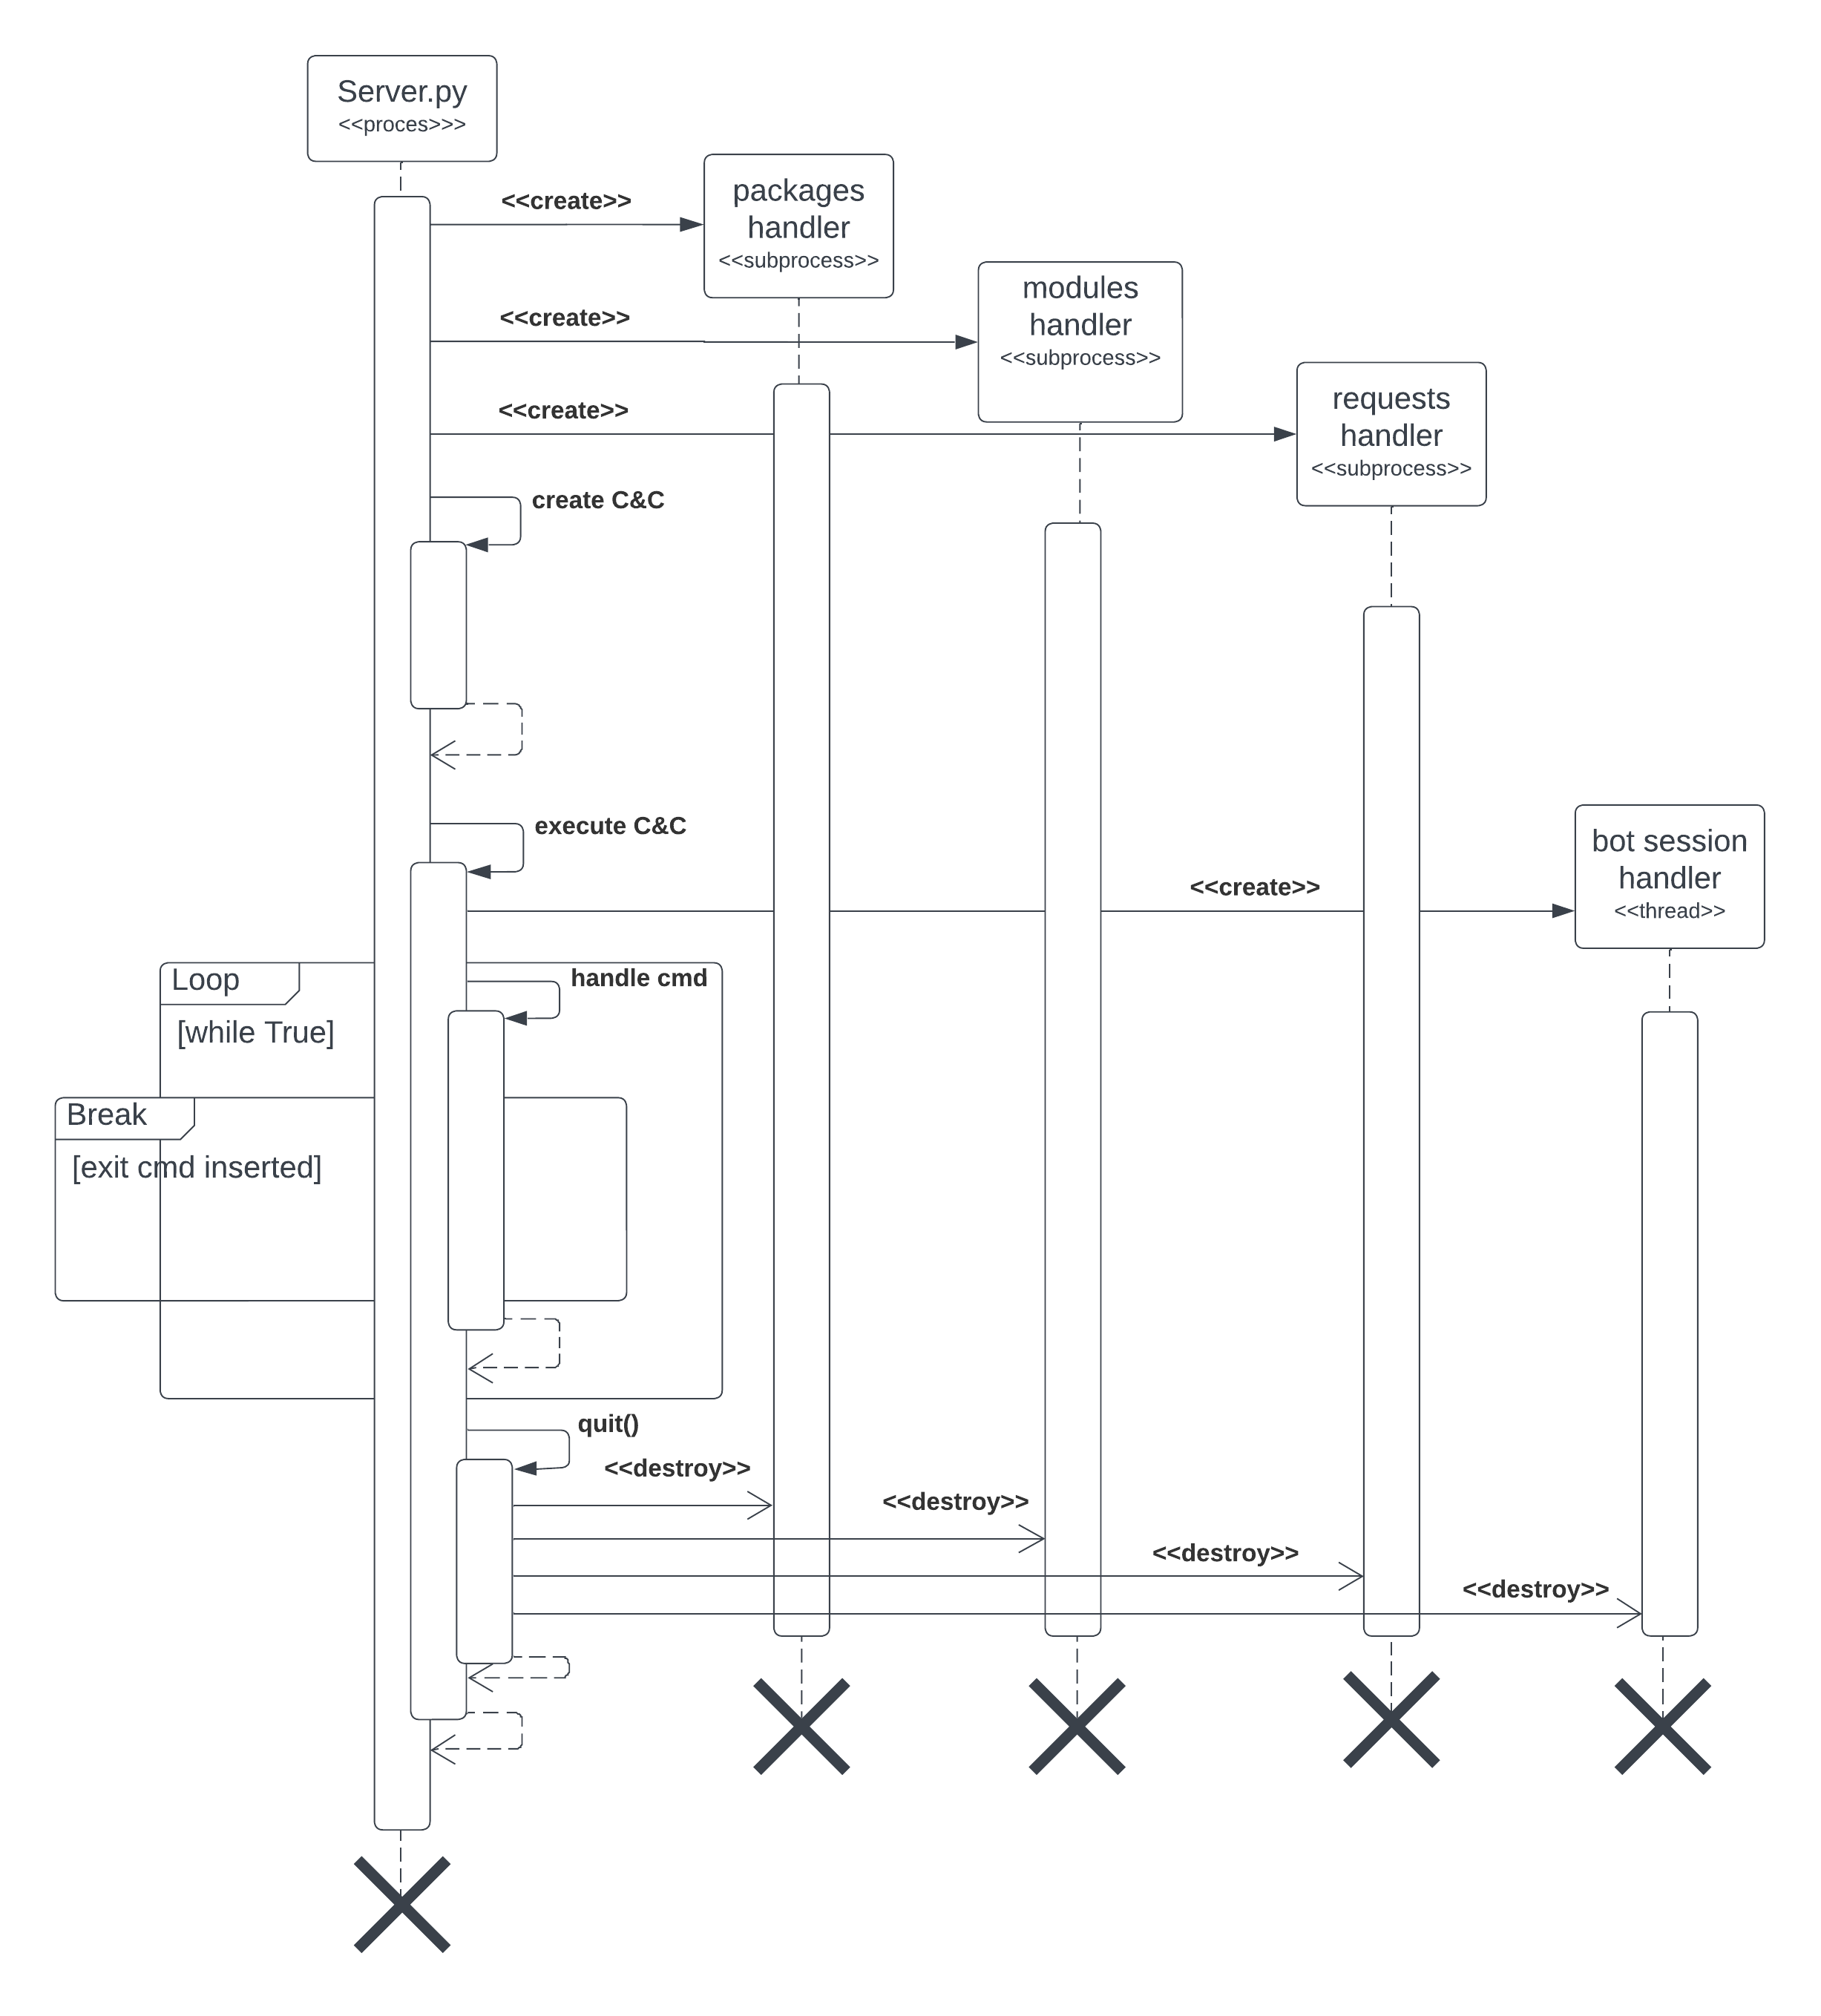
\includegraphics[width=\textwidth]{res/fig/byob-uml-server.png}
    \caption{Diagramma di sequenza di Byob.}
    \label{fig:byobumlserver}
\end{figure}


\subsection{Payload}

L'infezione attraverso payload è strutturata su più parti consequenziali.

Il file che la vittima esegue è il \textit{Dropper}.
Il Dropper scarica dal server lo Stager e lo esegue. Le righe di codice Python reponsabili del download sono inizialmente serializzate,compresse e codificate in base64, per rendere più difficile l'identificazione di codice malevolo da parte strumenti di rilevazione.

Lo Stager, a sua volta, scarica il Payload dal server.  Di default il server invia il payload in chiaro, ma è possibile criptare il contenuto del Payload, in questo caso lo Stager si preoccupa di decriptarlo prima di eseguirlo.

Il Payload è il cuore del malware.

Una volta eseguito instaura una connessione col Server e inizializza due thread, incaricati di ricercare e importare  moduli e packages da remoto, per poi entrare in un loop in attesa di task da eseguire.

Alla ricezione di un task,  esegue il parsing e ne esegue comando, cui  risultato viene incapsulato ed inoltrato al server.
Nel caso il server operi  senza interfaccia web, viene eseguito un thread incaricato di eseguire polling verso il server, a cui il server occasionalmente risponderà con un task.

In caso la ricezione del comando fosse un modulo, questo viene importato da remoto ed inseguito eseguito.

L'importazione di un modulo (o package) avviene aggiungendo un oggetto di classe Loader, contenenti i metodi \textit{find\_module} e \textit{load\_module}, alla lista di oggeti \textit{sys.meta\_path} ed in seguito eseguendo l'import manuale del modulo. 
Normalmente, quando l'interprete Python cerca di importare un modulo, naviga la lista \textit{sys.meta\_path} ed esegue il metodo \textit{find\_module} di ciascun oggetto. Questo metodo restituisce un loader del modulo selezionato nel caso lo trovi. Un loader è un oggetto che implementa il metodo \textit{load\_module}.
Una volta che il loader è stato trovato, ne viene eseguito il metodo \textit{load\_module} che importa il modulo all'interno del contesto.

Byob sfrutta questo meccanismo. Quando esegue l'import manuale di un modulo remoto, l'interprete si imbatte nel loader inserito da Byob all'interno della lista \textit{sys.meta\_path} ed esegue il suo metodo di ricerca. Questo cerca il modulo all'interno della lista di moduli disponibili precedentemente estratta dal server, e nel caso lo trovi ritorna un'istanza di se stesso. Dato che la classe loader di Byob è fornita anche del metodo \textit{load\_module}, può eseguirlo per importare il modulo da remoto.


Quando il bot è incaricato di eseguire l'upload di un file verso il server, invia una richiesta POST al sottoprocesso del server, incaricato di gestire le richieste POST, sulla porta dedicata.

\section{Testing e debug}
Per eseguire il testing, il Server è stato Containerizzato con Docker.
Il build dell'immagine è stato eseguito attraverso il seguente Dockerfile:
\lstset{  basicstyle=\footnotesize,
frame=single}
\begin{lstlisting}[caption={Byob Server Dockerfile},label={listing-byobdocker},frame=single]
FROM ubuntu:bionic

WORKDIR /app
COPY . .
RUN apt-get update && \
    apt-get upgrade -y && \
    apt-get install -y build-essential cmake && \
    apt-get install -y python3.6 python3-pip && \

WORKDIR /app/web-gui
RUN python3.6 -m pip install pip --upgrade && \
    python3.6 -m pip install -r requirements.txt && \
    rm -rf .gitignore .travis.yml README.md requirements.txt \
        startup.sh docker-pyinstaller*

EXPOSE 5000 1337 1338 1339
ENTRYPOINT python3.6 run.py --debug
\end{lstlisting}
Il Dockerfile specifica che al momento del build deve essere copiato il sorgente del Server all'interno del container, che devono essere installate tutte le dipendenze necessarie e che devono essere esposte le porte 5000, 1337, 1338, 1339 del Container.
Per eseguire  il container contenente il server è stato utilizzato  il seguente \textit{bash} script:
\begin{lstlisting}
containers=`docker ps -a | grep -A 1 byob | cut -b -12`;
for x in $containers; do 
    docker stop $x && docker rm $x ;
done;
docker run --name byob-web -it  -p 5000:5000 -p 1337:1337 \
    -p 1338:1338 -p 1339:1339 -v ./byob:/app   byobserver ;
\end{lstlisting}
Lo script interrompe l'esecuzione di tutti i container Byob esistenti e li rimuove prima di eseguire un nuovo container. La porta 5000 dell'host viene mappata alla porta del C\&C  mentre le restanti sono mappate ai servizi di distribuzione dei moduli/packages e    gestione delle richieste POST. La directory contenente il sorgente è stata mappata ad una directory dell'host in modo che fosse facile modificarne il codice all'occorrenza e per fare in modo che alla rimozione del container la directory fosse persistente sulla macchina host. Gli argomenti \textit{-it} sono utilizzati per rendere possibile l'interazione con la shell di debug del container.

Purtroppo il software ha presentato diversi problemi e bug da risolvere nella sua versione \textit{out of the box}. 

La funzionalità di import dei   packages da remoto risulta rotta. In particolare la ricerca confonde i moduli con i packages,  non riusciendo quindi mai a trovare ciò che si desidera poi importare. Il problema è stato aggirato ma non risolto, evitando di perdere troppo tempo su questioni secondarie, importando manualmente da locale i packages necessari.

I moduli di post-exploitation sono compatibili solo con alcuni degli OS e la maggior parte risultava non funzionante. 
La botnet è stata testata sia con bot Windows che con bot Linux.
Tra i mooduli  testati e non funzionanti vi sono i moduli per eseguire screenshots, keylogging, cattura del traffico di rete ed uso della  Webcam.

Analizzando il modulo Keylogger si può notare che il modulo risulta scritto in modo errato, forse perché utilizza una versione deprecata di API della libreria che sfruttava per eseguire il suo compito. 

Tra i moduli che invece risultano funzionanti vi erano quello utilizzato per eseguire scansioni delle porte di rete e quello per la gestione dei processi.

Le funzionalità di RAT funzionano correttamente.
In particolare è stata testata l'esecuzione di codice python arbitrario attraverso riga di comando o  attraverso l'import di moduli creati appositamente.

La  creazione del Payload criptato non funziona correttamente.


Le funzionalità di geolocalizzazione, l'import di script di Google Analytics e font scaricati da Internet sono stati rimossi in quanto si appoggiano a servizi web esterni non raggiungibili dall'interno del perimetro di testing, provocando crash dell'applicativo e ritardi nell'esecuzione.



A seguito di una fase di risoluzione dei problemi che ha richiesto un considerevole impiego di tempo, si è ritenuto opportuno procedere alla verifica con IDS delle sole funzionalità che al momento risultavano operative, per poi procedere con lo studio di un'ulteriore Botnet.

\chapter{Rilevazioni con IDS}
In \Cref{fig:byob-result-1} si possono vedere gli eventi generati da Security Onion attraverso il modulo Suricata al momento dell'esecuzione del Payload. Gli eventi sono autoesplicativi e fanno riferimento in particolare a:
\begin{itemize}
    \item Download di eseguibile;
    \item Richiesta web verso indirizzo IP;
    \item Rilevazione di Python all'interno dello user-agent;
    \item Rilevazione di codice di classe Loader di Byob;
    \item Rilevazione di codice di Stager di Byob.
\end{itemize}

Gli eventi più significativi fanno riferimento alla rilevazione di eseguibili e codici maligno noto. Se il download del payload fosse stato criptato nessuna di queste rilevazioni   avrebbe avuto luogo tranne il riferimento all'indirizzo IP.
\begin{figure}[hbtp]
    \centering
    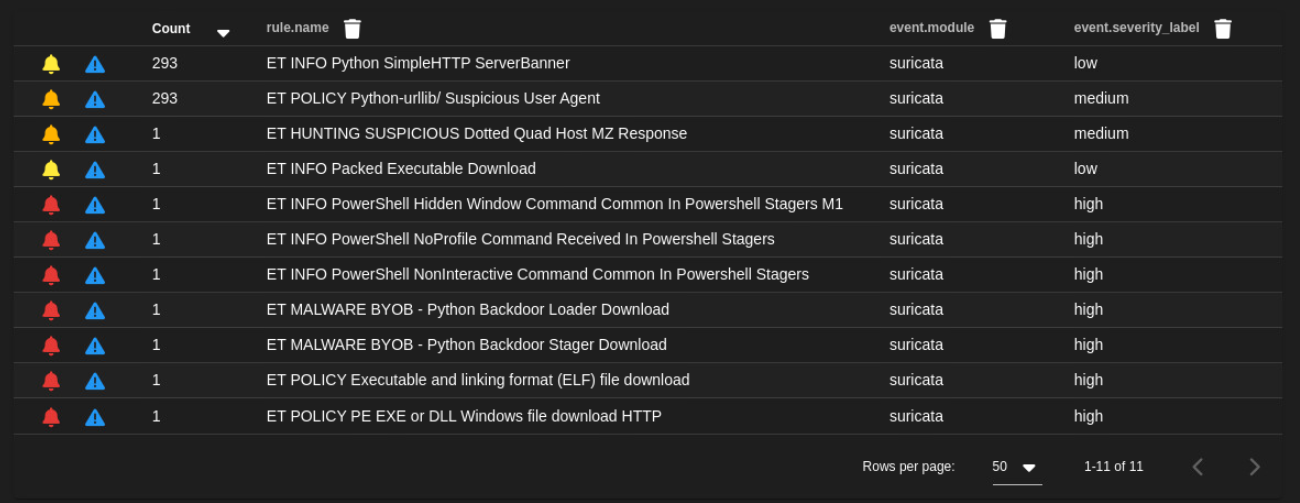
\includegraphics[width=\textwidth]{res/fig/byob-result-1.png}
    \caption{Rilevazione Security Onion dell'esecuzione del Payload.}
    \label{fig:byob-result-1}
\end{figure}


In \Cref{fig:byob-results-2-3} si possono osservare le rilevazioni di Security Onion e Ossim in merito all'esecuzione del modulo di scansione di rete.

Le funzionalità di RAT attraverso reverse-shell e l'utilizzo di moduli Python generici costruiti ad-hoc non sono stati rilevati.
Questo perché  Suricata non ha fingerprints che facciano riferimento ai moduli da noi creati, mentre i comandi inoltrati attraverso reverse-shell sono criptati con AES-256 e non vi è modo di identificare quel traffico di rete come maligno sfruttando solo SIDS.
%inserire test con import di miner che strelka dovrebbe rilevare specificando che import non è criptato e quindi può leggere.

\begin{figure}[hbtp]
    \centering
    \begin{subfigure}{\textwidth}
        \centering
        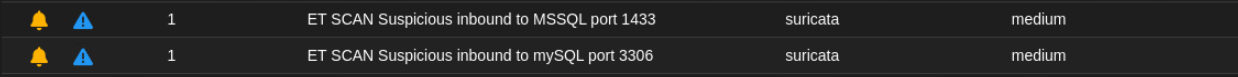
\includegraphics[width=\textwidth]{res/fig/byob-result-2.png}
        \caption{Security Onion}
        \label{fig:byob-result-2}
    \end{subfigure}
    \hfill
    \begin{subfigure}{\textwidth}
        \centering
        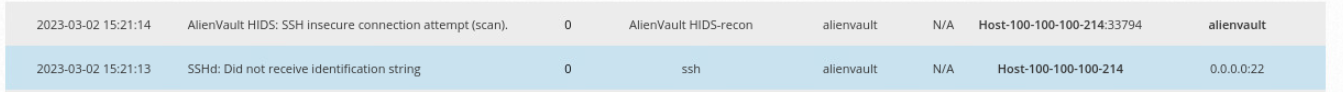
\includegraphics[width=\textwidth]{res/fig/byob-result-3.png}
        \caption{Ossim}
        \label{fig:byob-result-3}
    \end{subfigure}
    \caption{Rilevazioni della scansione di rete eseguita da bot attraverso modulo apposito.}
    \label{fig:byob-results-2-3}
\end{figure}


  \appendix
  \begin{appendices}
  
\end{appendices}


  \backmatter{}
  \nocite{*}            % aggiunge tutti i riferimenti nel .bib (anche non citati)
\printbibliography[%  % produce la bibliografia
  heading=bibintoc    % inserisce il titolo nell'indice generale
]

  \chapter{Ringraziamenti}
Desidero innanzitutto  esprimere la mia gratitudine al  relatore, il Dott. Gabriele D'Angelo, e al correlatore, il Dott. Ciro Barbone, per la loro eccezionale disponibilità e competenza, che mi hanno permesso di vivere un'esperienza di tesi estremamente gratificante e motivante.
 
Un ringraziamento speciale alla mia famiglia, per tutto quello che fanno per me, per il loro affetto  e appoggio incondizionato.
 
 Ringrazio di cuore Veronika, che in questo ultimo anno mi è sempre stata  vicina, supportandomi  e spronandomi anche durante le nottate di studio più matte e disperate.

 Ringrazio Cicio, Lino, Vago e Salmon per essere ed essere stati al mio fianco.
 
 Infine, desidero esprimere la mia gratitudine verso i miei amici, coloro che sono sempre  al mio fianco e quelli che, nonostante il tempo e la distanza, so che ci saranno sempre.
 

\end{document}
